
\part{DAĞITIK ALGILAYICI AĞI TASARIM VE SİMÜLASYON SONUÇLARI}


%\part{OPNET İLE YENİLENEBİLİR ENERJİ SİSTEMİ İÇİN DAĞITIK SENSÖR AĞI TASARIM VE SİMÜLASYON SONUÇLARI}
\thispagestyle{empty}
\newpage
\section{LAN TASARIM VE SİMÜLASYON SONUÇLARI}
\subsection{OPNET Yerel Ağ Tasarımı} \label{opnetges}

\begin{figure}[htbp]
\centerline{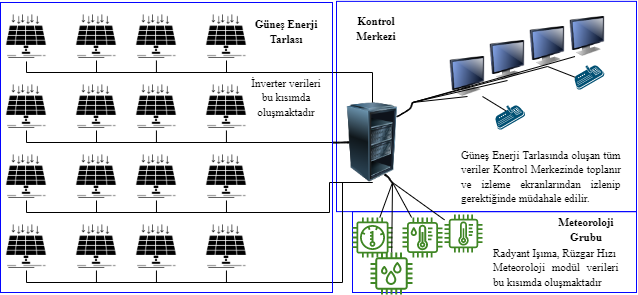
\includegraphics[width=\columnwidth]{Resim/PV-2.png}}
\caption{Güneş enerji sistemi haberleşme topolojisi}
\label{fig:4-6}
\end{figure}

Şekil \ref{fig:4-6}’da sahada kurulu olarak çalışan güneş enerji panelleri ve hava durumu algılayıcılarının sistem odasında bulunan sunucuyla bağlantısı ve sunucu ile komuta kontrol merkezinde bulunan görüntüleme bilgisayarları arasındaki bağlantının topolojisi gösterilmiştir. İlgili topoloji sadece yerel ağı gösteren bir topoloji olduğu unutulmamalıdır. \gls{wan} tasarımı hakkında yapılan çalışmalar, ayrı bir başlıkta incelenmiştir.

\subsubsection{Ethernet Teknolojisi \gls{lan} Tasarımı}\label{yerelEthernet}


\paragraph{Güneş Enerji Sistemi \gls{lan} Tasarımı }

\begin{figure}[htbp]
\centerline{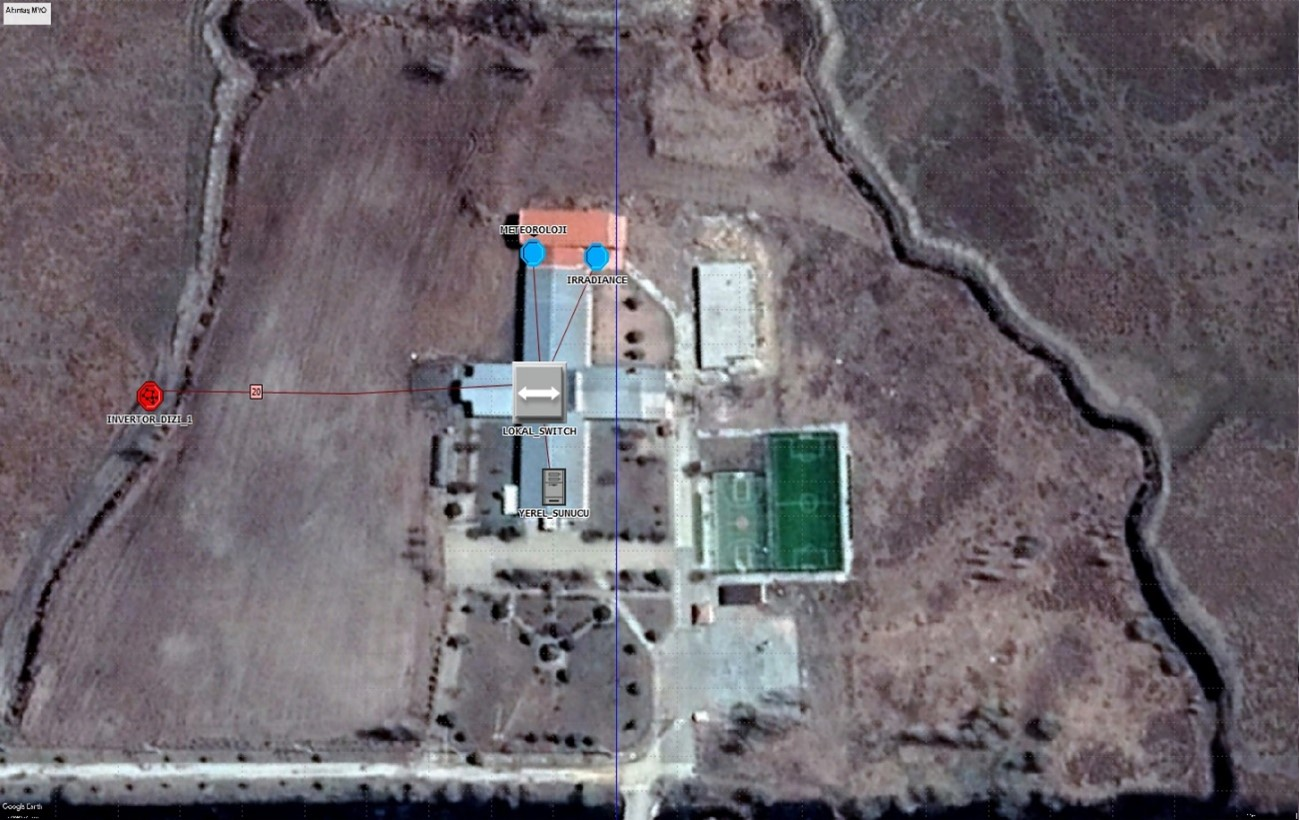
\includegraphics[width=\columnwidth]{Resim/Sekil4-7.jpg}}
\caption{Altıntaş \gls{myo}'nun OPNET yazılımda tasarım topolojisi.}
\label{fig:4-7}
\end{figure}

Bölüm \ref{opnetges}'deki ilgili tabloda güneş enerji sisteminde kullanılan algılayıcılara göre OPNET yazılımında oluşturulan ağın görseli Şekil \ref{fig:figure9}'dedir. İlgili ağ yapısının tasarımı için OPNET yazılımında seçilmiş Ethernet algılayıcı düğümünün detayı şekil \ref{fig:4-9}’da gösterilmiştir. Bölüm \ref{algilayicidugum}'de tanımlanan Ethernet düğüm modülü ile OPNET yazılımında düğüm modülü uyumluluk göstermektedir.

Yerel enerji üretim durumunu kontrol edebilmek için komuta kontrol merkezi ile enerji üretim sisteminin haberleşme gecikmesinin 1 saniyenin altında olması ve paket trafiğinin minimum gecikmeyle komuta merkezine aktarılması gerektiği \gls{iec} 61724 standardının temel kriteridir. Bu kritere göre tasarlanan topolojide gözlemlenen performans değerleri Şekil \ref{fig:4-10}--\ref{fig:4-12}’lerde paylaşılmıştır.


\begin{figure}[htbp]
\centerline{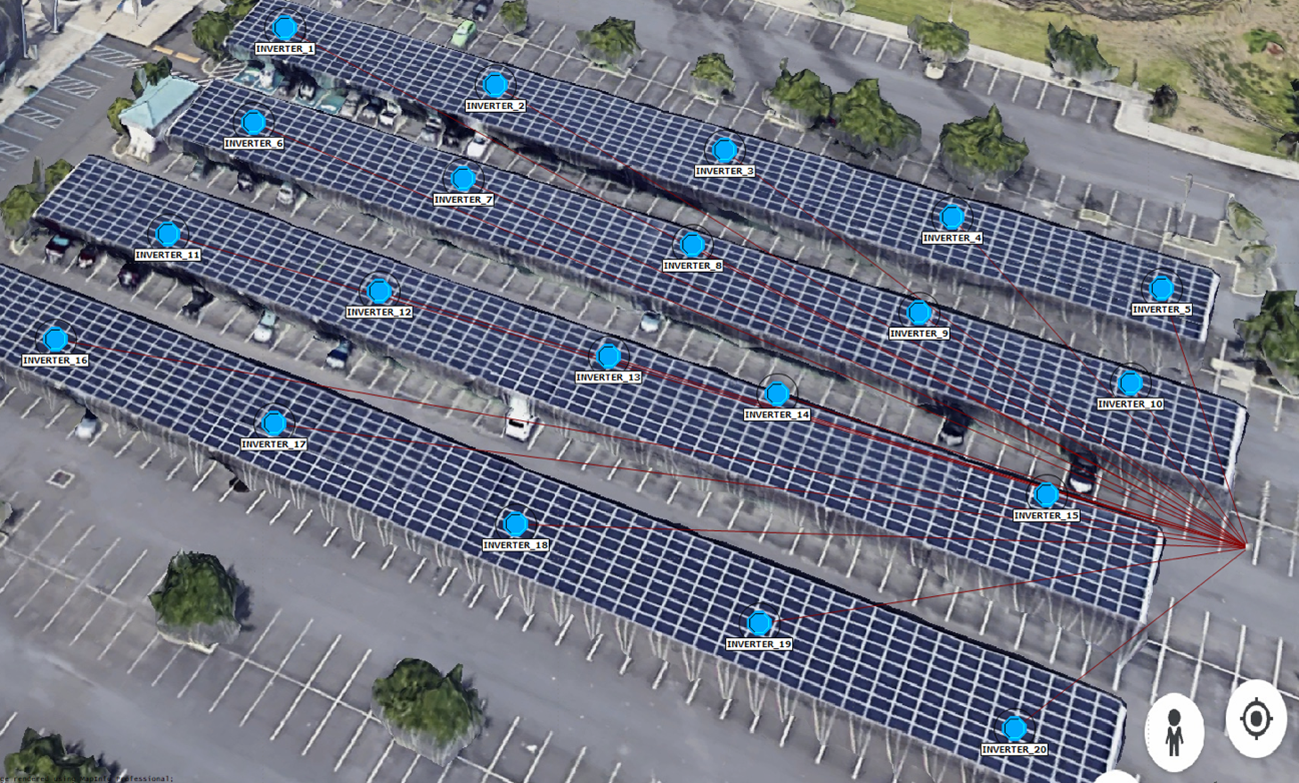
\includegraphics[width=10cm]{Resim/Sekil 4-8.png}}
\caption{Kampüs ortamında kurulan örnek güneş enerji santralinin invertör dizi grubunun OPNET yazılımında tasarlanması.}
\label{fig:4-8}
\end{figure}

\begin{figure}[htbp]


\centerline{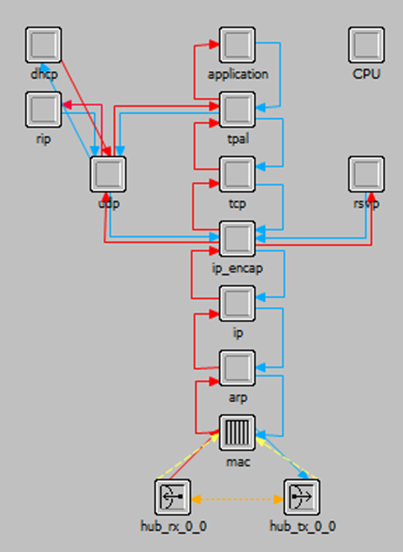
\includegraphics[width=7cm]{Resim/Sekil4-9.png}}
\caption{OPNET yazılımında tasarlanan ethernet tipi algılayıcıların görüntüsü.}
\label{fig:4-9}
\end{figure}
\begin{comment}
%ESKİ ŞEKİL SİLEBİLİRSİN
\begin{figure}[htbp]
\centerline{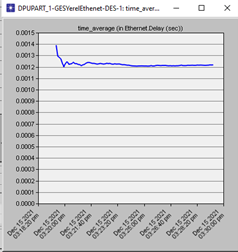
\includegraphics[width=5cm]{Resim/sekil4-10.png}}
\caption{\gls{lan}'da ethernet haberleşmesinde gözlemlenen gecikme değişimi.}
\label{fig:4-10}
\end{figure}
\end{comment}



\begin{figure}[htbp]
\centering
%ethernet haberleşmesinde LAN gecikme grafiğidir
\pgfplotsset{every axis/.append style={
font=\footnotesize,
thin,
tick style={ultra thin}},
scaled y ticks=false,
yticklabel style = {
/pgf/number format/fixed,
/pgf/number format/precision=5
},
}

    \begin{tikzpicture}
    \begin{axis}[
    xlabel={Simülasyon Süresi (Saniye)},
    ylabel={Uçtan Uca Gecikme (Saniye)},
    grid,
    legend style = {font=\tiny,at={(1,0.8)}, anchor=east}
    ]

\addplot [color=cyan, mark=star, mark repeat =14, mark size = 3]  table [x = timesec, y = GESYerelEthenetEthernetDelaysec, col sep = comma] {yedek.csv};
%\addlegendentry{Ethernet bağlantı gecikme değeri}



\end{axis}
\end{tikzpicture}
\caption{\gls{lan}'da ethernet haberleşmesinde gözlemlenen gecikme değişimi.}
\label{fig:4-10}
\end{figure}




\begin{comment}

\begin{figure}[htbp]
\centerline{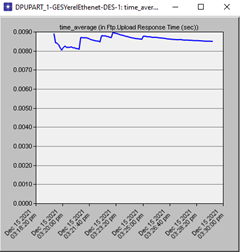
\includegraphics[width=5cm]{Resim/sekil4-11.png}}
\caption{\gls{lan}'da algılayıcılardan gönderilen verilerin yerel sunucuya yüklenme süresi}
\label{fig:4-11}
\end{figure}
\end{comment}

\begin{figure}[htbp]


\centering
%ethernet haberleşmesinde LAN gecikme grafiğidir
\pgfplotsset{every axis/.append style={
font=\footnotesize,
thin,
tick style={ultra thin}},
scaled y ticks=false,
yticklabel style = {
/pgf/number format/fixed,
/pgf/number format/precision=5
},
}

    \begin{tikzpicture}
    \begin{axis}[
    ylabel={Veri Yükleme Süresi (Saniye)},
    xlabel={Simülasyon Süresi (Saniye)},
    grid,
    legend style = {font=\tiny,at={(1,0.8)}, anchor=east}
    ]

\addplot [color=red, mark=star, mark repeat =14, mark size = 3]  table [x = timesec, y = GESYerelEthenetFtpUploadResponseTimesec, col sep = comma] {yedek.csv};
%\addlegendentry{Ethernet bağlantı gecikme değeri}



\end{axis}
\end{tikzpicture}


\caption{\gls{lan}'da algılayıcılardan gönderilen verilerin yerel sunucuya yüklenme süresi}
\label{fig:4-11}
\end{figure}



\begin{figure}[htbp]
%\centerline{\includegraphics[width=5cm]{Resim/şekil4-12.png}}
\centering
\pgfplotsset{every axis/.append style={
font=\footnotesize,
thin,
tick style={ultra thin}},
}
    \begin{tikzpicture}
\begin{semilogyaxis}[ymax = 20000.0000000,
xlabel={Simülasyon Süresi (Saniye)},
ylabel={Yüklenen Veri Boyutu (Byte/s)},
xmode=normal, ymode=log, 
grid = major,
log ticks with fixed point,
ytick={6,10,200,14400},
transpose legend,
legend columns = 2,
legend style = {font=\tiny,at={(1,0.8)}, anchor=east}
]


\addplot [color=blue, mark=oplus*, mark repeat =14, mark size = 3]  table [x = Simulation Duration, y = Received Current Data, col sep = comma] {fig4deneme (1).csv};


%--
\addplot [color=yellow, mark=pentagon*, mark repeat =14, mark size = 3, mark phase = 8]  table [y = Received Voltage Data, col sep = comma] {fig4deneme (1).csv};

%--

\addplot [color = green, dotted, mark=diamond*, mark repeat =14, mark size = 3, ]table [y = METEOR, col sep = comma] {fig4deneme (1).csv};

%--
\addplot [color=orange, mark=square*, mark repeat =14, mark size = 3]table [y = Received Wind Speed Data, col sep = comma] {fig4deneme (1).csv};

%---
\addplot [color=violet, mark=triangle*, mark repeat =14, mark size = 3] table [y = Received Global Irradiance Data, col sep = comma] {fig4deneme (1).csv};


\legend{İnverter Gerilim,İnverter Akım,Rüzgar Hızı,Meteoroloji,Radyant Işıma}


\end{semilogyaxis}
\end{tikzpicture}
\caption{\gls{lan}'da 1 adet \gls{myo}'ya ait yerel sunucuya yüklenen veri grubunun değişimi}
\label{fig:4-12}
\end{figure}




\newpage


\paragraph{Rüzgar Enerji Sistemi LAN Tasarımı}

Ethernet haberleşmesinde \gls{utp} kablolamanın en büyük sıkıntısı mesafedir. 
Veri aktarımında 100 metrede 24,6dB güç kaybı olmasından dolayı mutlaka cihaz aralarına güçlendirici kullanılması gerekir \cite{yilmazanalysis}. Tezde model olarak kullanılan rüzgar türbinlerinin yüksekliği 80 metredir \cite{bauer_2010}.
Algılayıcı düğüm modüllerinden gelen Ethernet kabloları türbinin zemininde bulunan bir toplayıcı anahtara gelmektedir. Toplayıcı anahtar ile lokal sunucunun olduğu komuta merkezindeki yönetim anahtarına \gls{utp} kablo bağlantısı vardır. Farklı kablo altyapıları kullanılarak haberleşme sağlanabilir örnek olarak fiber optik kablosu seçildiğinde optik kablo için Ethernet anahtarı arasına konulacak bir fiber dönüştürücü modül ve fiber kablolarının füzyon eki ile sonlandırma kutusu ve yan ekipmanlarına ihtiyaç duyulacaktır. Bu tasarımın getireceği ekstra malzemeler bir maliyet unsuru oluşturacağından sadece \gls{utp} kablolama ile çözüme gidilme tercihi kabul edilmiştir.

\begin{figure}[htbp]
%\centerline{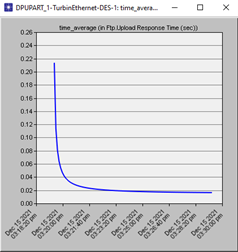
\includegraphics[width=6cm]{Resim/sekil4-13.png}}
\centering
%ethernet haberleşmesinde LAN gecikme grafiğidir
\pgfplotsset{every axis/.append style={
font=\footnotesize,
thin,
tick style={ultra thin}},
scaled y ticks=false,
yticklabel style = {
/pgf/number format/fixed,
/pgf/number format/precision=5
},
}

    \begin{tikzpicture}
    \begin{axis}[
    xlabel={Simülasyon süresi (Saniye)},
    ylabel={Veri Yükleme Süresi (Saniye)},
    grid,
    legend style = {font=\tiny,at={(1,0.8)}, anchor=east}
    ]

\addplot [color=red, mark=star, mark repeat =14, mark size = 3]  table [x = Simulation Duration, y = TurbinUploadResponseTime, col sep = comma] {fig4deneme (1).csv};
%\addlegendentry{Ethernet bağlantı gecikme değeri}



\end{axis}
\end{tikzpicture}


\caption{Algılayıcılardan gönderilen verilerin yerel sunucuya yüklenme süresi}
\label{fig:4-13}
\end{figure}


\begin{figure}[htbp]
%\centerline{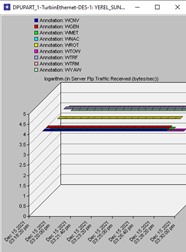
\includegraphics[width=5cm]{Resim/sekil4-14.png}}

\centering
\pgfplotsset{every axis/.append style={
font=\footnotesize,
thin,
tick style={ultra thin}},
}
    \begin{tikzpicture}
\begin{semilogyaxis}[ymax = 20000.0000000,
xlabel={Simülasyon Süresi (Saniye)},
ylabel={Yüklenen Veri Boyutu (Byte/s)},
xmode=normal, ymode=log, 
grid = major,
log ticks with fixed point,
ytick={15004,14004,8000,11008,12010,2006,8006,12016,6004},
transpose legend,
legend columns = 3,
legend style = {font=\tiny,at={(1,0.3)}, anchor=east}
]


\addplot [color=blue, mark=oplus*, mark repeat =14, mark size = 3]  table [x = Simulation Duration, y = WCNV, col sep = comma] {fig4deneme (1).csv};


%--
\addplot [color=yellow, mark=pentagon*, mark repeat =14, mark size = 3, mark phase = 8]  table [y = WGEN, col sep = comma] {fig4deneme (1).csv};

%--

\addplot [color = green, dotted, mark=diamond*, mark repeat =14, mark size = 3, ]table [y = WMET, col sep = comma] {fig4deneme (1).csv};

%--
\addplot [color=orange, mark=square*, mark repeat =14, mark size = 3]table [y = WNAC, col sep = comma] {fig4deneme (1).csv};

%---
\addplot [color=violet, mark=triangle*, mark repeat =14, mark size = 3] table [y = WROT, col sep = comma] {fig4deneme (1).csv};

%--
\addplot [color=yellow, mark=pentagon*, mark repeat =14, mark size = 3, mark phase = 8]  table [y = WTOW, col sep = comma] {fig4deneme (1).csv};


%--
\addplot [color=black, mark=pentagon*, mark repeat =14, mark size = 1, mark phase = 8]  table [y = WTRF, col sep = comma] {fig4deneme (1).csv};

%--
\addplot [color=orange, mark=pentagon*, mark repeat =14, mark size = 1, mark phase = 8]  table [y = WTRM, col sep = comma] {fig4deneme (1).csv};


%--
\addplot [color=cyan, mark=pentagon*, mark repeat =14, mark size = 1, mark phase = 8]  table [y = WYAW, col sep = comma] {fig4deneme (1).csv};
\legend{WCNV , WGEN , WMET , WNAC , WROT , WTOW , WTRF , WTRM , WYAW}
\end{semilogyaxis}



\end{tikzpicture}



\caption{Yerel sunucuya yüklenen veri grubunun logaritmik değeri}
\label{fig:4-14}
\end{figure}

\begin{figure}[htbp]
%\centerline{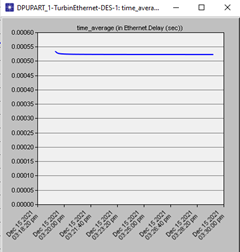
\includegraphics[width=5cm]{Resim/sekil4-15.png}}

\centering
%ethernet haberleşmesinde LAN gecikme grafiğidir
\pgfplotsset{every axis/.append style={
font=\footnotesize,
thin,
tick style={ultra thin}},
scaled y ticks=false,
yticklabel style = {
/pgf/number format/fixed,
/pgf/number format/precision=5
},
}

    \begin{tikzpicture}
    \begin{axis}[
    xlabel={Simülasyon Süresi (Saniye)},
    ylabel={Uçtan Uca Gecikme (Saniye)},
    grid,
    legend style = {font=\tiny,at={(1,0.8)}, anchor=east}
    ]

\addplot [color=red, mark=star, mark repeat =14, mark size = 3]  table [x = Simulation Duration, y = turbinEthernetDelay, col sep = comma] {fig4deneme (1).csv};
%\addlegendentry{Ethernet bağlantı gecikme değeri}



\end{axis}
\end{tikzpicture}
\caption{Ethernet haberleşmesinde yaşanan gecikme}
\label{fig:4-15}
\end{figure}

Yerel enerji üretim durumunu kontrol edebilmek için komuta kontrol merkezi ile enerji üretim sisteminin haberleşme gecikmesinin 1 saniyenin altında olması ve paket trafiğinin minimum gecikmeyle komuta merkezine aktarılması gerektiği \gls{iec} 61400-25 standardının temel kriteridir. Bu kritere göre tasarlanan topolojinin performans değerleri Şekil \ref{fig:4-13}--\ref{fig:4-15}’de paylaşılmıştır.
\newpage  %BUNUN AMACI SAYFAYI DÜZGÜN ÇIKARTMAK İÇİN ÇÜNKÜ BAŞKA BİR SECTİON'UN ALTINDA ÖNCEKİ SECTİONA AİT RESİMLERİ ÇIKARTIYORDU
\subsubsection{\gls{wifi} Teknolojisi \gls{lan} Tasarımı}\label{yerelWifi}

\paragraph{Güneş Enerji Sistemi \gls{lan} Tasarımı}

\gls{wifi} altyapısında \gls{ges}'in maliyet ve performans değerleri ile Altıntaş \gls{myo}’nun OPNET ortamında simülasyon raporları bu bölümde paylaşılmıştır.


\begin{figure}[htbp]
\centerline{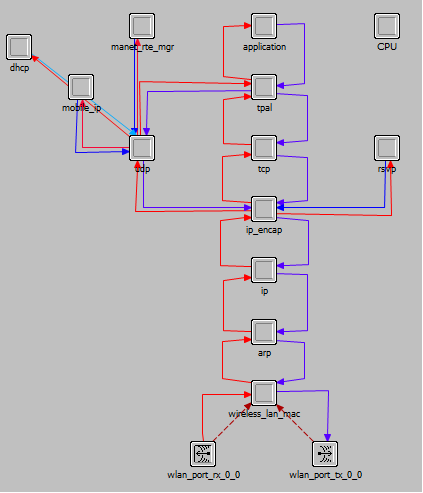
\includegraphics[width=7cm]{Resim/PV-Sayfa -5.drawio.png}}
\caption{OPNET yazılımındaki \gls{wifi} algılayıcı düğümünün gösterimi.}
\label{fig:4-16}
\end{figure}


Yerel enerji üretim durumunu kontrol edebilmek için komuta kontrol merkezi ile enerji üretim sisteminin haberleşme gecikmesinin 1 saniyenin altında olması ve paket trafiğinin minimum gecikmeyle komuta merkezine aktarılması gerektiği \gls{iec} 61724 standardının temel kriteridir. Bu kritere göre tasarlanan topolojinin performans değerleri Şekil \ref{fig:4-17}--\ref{fig:4-19}’da paylaşılmıştır

\begin{figure}[htbp]
%\centerline{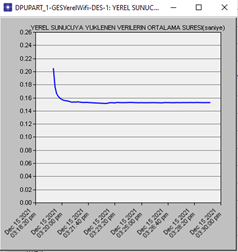
\includegraphics[width=5cm]{Resim/sekil4-16.png}}

\centering
%ethernet haberleşmesinde LAN gecikme grafiğidir
\pgfplotsset{every axis/.append style={
font=\footnotesize,
thin,
tick style={ultra thin}},
scaled y ticks=false,
yticklabel style = {
/pgf/number format/fixed,
/pgf/number format/precision=5
},
}

    \begin{tikzpicture}
    \begin{axis}[
    xlabel={Simülasyon süresi (Saniye)},
    ylabel={Veri Yükleme Süresi (Saniye)},
    grid,
    legend style = {font=\tiny,at={(1,0.8)}, anchor=east}
    ]

\addplot [color=red, mark=star, mark repeat =14, mark size = 3]  table [x = Simulation Duration, y = WifiYerelUploadTime, col sep = comma] {fig4deneme (1).csv};
%\addlegendentry{Ethernet bağlantı gecikme değeri}



\end{axis}
\end{tikzpicture}



\caption{Yerel sunucuya yüklenen verilerin ortalama süresi}
\label{fig:4-17}
\end{figure}


\begin{figure}[htbp]
%\centerline{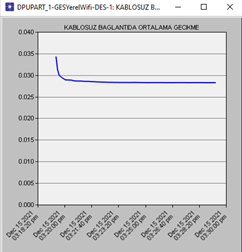
\includegraphics[width=5cm]{Resim/sekil4-17.png}}

\centering
%ethernet haberleşmesinde LAN gecikme grafiğidir
\pgfplotsset{every axis/.append style={
font=\footnotesize,
thin,
tick style={ultra thin}},
scaled y ticks=false,
yticklabel style = {
/pgf/number format/fixed,
/pgf/number format/precision=5
},
}

    \begin{tikzpicture}
    \begin{axis}[
    xlabel={Simülasyon Süresi (Saniye)},
    ylabel={Uçtan Uca Gecikme (Saniye)},
    grid,
    legend style = {font=\tiny,at={(1,0.8)}, anchor=east}
    ]

\addplot [color=cyan, mark=star, mark repeat =14, mark size = 3]  table [x = Simulation Duration, y = wirelessGESDelay, col sep = comma] {fig4deneme (1).csv};
%\addlegendentry{Ethernet bağlantı gecikme değeri}



\end{axis}
\end{tikzpicture}
\caption{Yerel ağda yaşanan gecikme süresi}
\label{fig:4-18}
\end{figure}

İlgili simülasyon sonuçlarına göre güneş enerji santralinin haberleşme standartlarında bir ihlal durumu olmadan sağlıklı bir şekilde yerel sunucuya verilerin aktarıldığı gözlemlenmiştir.

\begin{figure}[htbp]
%\centerline{\includegraphics[width=5cm]{Resim/Sekil4-18.png}}
\centering
\pgfplotsset{every axis/.append style={
font=\footnotesize,
thin,
tick style={ultra thin}},
}
    \begin{tikzpicture}
\begin{semilogyaxis}[ymax = 20000.0000000,
xlabel={Simülasyon Süresi (Saniye)},
ylabel={Yüklenen Veri Boyutu (Byte/s)},
xmode=normal, ymode=log, 
grid = major,
log ticks with fixed point,
ytick={6,10,200,14400},
transpose legend,
legend columns = 2,
legend style = {font=\tiny,at={(1,0.8)}, anchor=east}
]


\addplot [color=blue, mark=oplus*, mark repeat =14, mark size = 3]  table [x = Simulation Duration, y = INVERTERAKIMwifiges, col sep = comma] {fig4deneme (1).csv};


%--
\addplot [color=yellow, mark=pentagon*, mark repeat =14, mark size = 3, mark phase = 8]  table [y =INVERTERVOLTAJwifiges, col sep = comma] {fig4deneme (1).csv};

%--

\addplot [color = green, dotted, mark=diamond*, mark repeat =14, mark size = 3, ]table [y = METEORwifiges, col sep = comma] {fig4deneme (1).csv};

%--
\addplot [color=orange, mark=square*, mark repeat =14, mark size = 3]table [y = RUZGARHIZIwifiges, col sep = comma] {fig4deneme (1).csv};

%---
\addplot [color=violet, mark=triangle*, mark repeat =14, mark size = 3] table [y = RADYANTISIMAwifiges, col sep = comma] {fig4deneme (1).csv};


\legend{İnverter Gerilim,İnverter Akım,Rüzgar Hızı,Meteoroloji,Radyant Işıma}


\end{semilogyaxis}
\end{tikzpicture}


\caption{Yerel sunucuya yüklenen veri gruplarının logaritmik değeri}
\label{fig:4-19}
\end{figure}

\paragraph{Rüzgar Enerji Sistemi \gls{lan} Tasarımı}

Domaniç \gls{myo}'nun rüzgar enerji sistemindeki haberleşme altyapısı \gls{wifi} olarak OPNET ortamında kurulduktan sonra edinilen simülasyon sonuçları Şekil \ref{fig:4-20}-\ref{fig:4-22}’de paylaşılmıştır.

\begin{figure}[htbp]
%\centerline{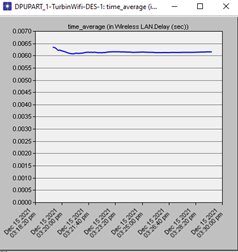
\includegraphics[width=5cm]{Resim/Sekil4-19.png}}


\centering
%ethernet haberleşmesinde LAN gecikme grafiğidir
\pgfplotsset{every axis/.append style={
font=\footnotesize,
thin,
tick style={ultra thin}},
scaled y ticks=false,
yticklabel style = {
/pgf/number format/fixed,
/pgf/number format/precision=5
},
}

    \begin{tikzpicture}
    \begin{axis}[
    xlabel={Simülasyon Süresi (Saniye)},
    ylabel={Uçtan Uca Gecikme (Saniye)},
    grid,
    legend style = {font=\tiny,at={(1,0.8)}, anchor=east}
    ]

\addplot [color=red, mark=star, mark repeat =14, mark size = 3]  table [x = Simulation Duration, y = WirelessLANDelaysecwifiLoc, col sep = comma] {fig4deneme (1).csv};
%\addlegendentry{Ethernet bağlantı gecikme değeri}



\end{axis}
\end{tikzpicture}


\caption{Yerel ağda yaşanan gecikme değişimi}
\label{fig:4-20}
\end{figure}

\begin{figure}[htbp]
%\centerline{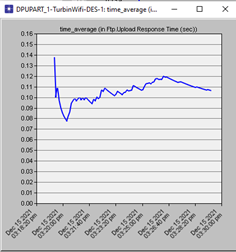
\includegraphics[width=5cm]{Resim/Sekil4-20.png}}

\centering
%ethernet haberleşmesinde LAN gecikme grafiğidir
\pgfplotsset{every axis/.append style={
font=\footnotesize,
thin,
tick style={ultra thin}},
scaled y ticks=false,
yticklabel style = {
/pgf/number format/fixed,
/pgf/number format/precision=5
},
}

    \begin{tikzpicture}
    \begin{axis}[
    xlabel={Simülasyon süresi (Saniye)},
    ylabel={Veri Yükleme Süresi (Saniye)},
    grid,
    legend style = {font=\tiny,at={(1,0.8)}, anchor=east}
    ]

\addplot [color=blue, mark=circle, mark repeat =14, mark size = 3]  table [x = Simulation Duration, y = FtpUploadResponseTimesecwifiLoc, col sep = comma] {fig4deneme (1).csv};
%\addlegendentry{Ethernet bağlantı gecikme değeri}



\end{axis}
\end{tikzpicture}


\caption{Yerel sunucuya yüklenen verilerin ortalama süre değerleri}
\label{fig:4-21}
\end{figure}


\begin{figure}[htbp]
%\centerline{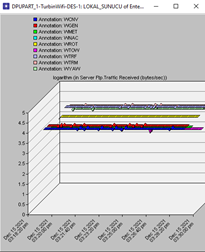
\includegraphics[width=5cm]{Resim/Sekil4-21.png}}

\centering
\pgfplotsset{every axis/.append style={
font=\footnotesize,
thin,
tick style={ultra thin}},
}
    \begin{tikzpicture}
\begin{semilogyaxis}[ymax = 20000.0000000,
xlabel={Simülasyon Süresi (Saniye)},
ylabel={Yüklenen Veri Boyutu (Byte/s)},
xmode=normal, ymode=log, 
grid = major,
log ticks with fixed point,
ytick={15004,14004,8000,11008,12010,2006,8006,12016,6004},
transpose legend,
legend columns = 3,
legend style = {font=\tiny,at={(1,0.3)}, anchor=east}
]


\addplot [color=blue, mark=oplus*, mark repeat =14, mark size = 3]  table [x = Simulation Duration, y = WCNV, col sep = comma] {fig4deneme (1).csv};


%--
\addplot [color=yellow, mark=pentagon*, mark repeat =14, mark size = 3, mark phase = 8]  table [y = WGEN, col sep = comma] {fig4deneme (1).csv};

%--

\addplot [color = green, dotted, mark=diamond*, mark repeat =14, mark size = 3, ]table [y = WMET, col sep = comma] {fig4deneme (1).csv};

%--
\addplot [color=gray, mark=square*, mark repeat =14, mark size = 3]table [y = WNAC, col sep = comma] {fig4deneme (1).csv};

%---
\addplot [color=brown, mark=triangle*, mark repeat =14, mark size = 3] table [y = WROT, col sep = comma] {fig4deneme (1).csv};

%--
\addplot [color=red, mark=triangle, mark repeat =14, mark size = 3, mark phase = 8]  table [y = WTOW, col sep = comma] {fig4deneme (1).csv};


%--
\addplot [color=black, mark=pentagon*, mark repeat =14, mark size = 1, mark phase = 8]  table [y = WTRF, col sep = comma] {fig4deneme (1).csv};

%--
\addplot [color=blue, mark=square, mark repeat =14, mark size = 1, mark phase = 8]  table [y = WTRM, col sep = comma] {fig4deneme (1).csv};


%--
\addplot [color=blue, mark=circle, mark repeat =14, mark size = 1, mark phase = 8]  table [y = WYAW, col sep = comma] {fig4deneme (1).csv};
\legend{WCNV , WGEN , WMET , WNAC , WROT , WTOW , WTRF , WTRM , WYAW}
\end{semilogyaxis}



\end{tikzpicture}




\caption{Yerel sunucuya yüklenen veri gruplarının değişimi}
\label{fig:4-22}
\end{figure}

\newpage
\subsubsection{Zigbee Teknolojisi ile \gls{lan} Tasarımı}\label{zigbee}


Zigbee haberleşme altyapısı \gls{wifi} ve ethernet haberleşme teknolojilerine göre çok daha ucuzdur fakat, \gls{iec}'nin belirlemiş olduğu gerçek zamanlı izleme standartlarına uymadığı gözlemlenmiştir. Önceki kısımlardaki gibi aynı noktalarda kurulan enerji sistemlerinin algılayıcı verilerinin oluşturmuş olduğu veri trafiğinin performans değerleri aşağıdaki başlıklarda gösterilmiştir.


\paragraph{Güneş Enerji Sistemi}\label{zigbeeges112}

\gls{lan}'da Zigbee teknolojisi enerji kullanım açısından çok verimlidir.
Fakat \gls{ieee} 1646 ve \gls{iec} 61850 standartlarınin belirlemiş olduğu gerçek zamanlı veri iletişim şartını sağlamamaktadır.
Resim \ref{fig:4-23}'de Zigbee ağının trafiğindeki gecikme değerleri görülmektedir. \gls{lan}'daki kabul edilebilir değerler 1 saniyenin altında olması gerekirken, Resim \ref{fig:4-23}'deki senaryoda dakika derecesinde bir gecikme yaşanmaktadır. \gls{wifi} ve Ethernet haberleşmesinde verinin rotalama metodu kullanılmasına karşın, Zigbee teknolojisinde bu özellik bulunmamaktadır. Resim \ref{fig:4-23}'deki gecikme sonucu olarak Resim \ref{fig:4-24}'da yerel sunucuya yüklenen veri boyutlarının 30.000 Byte/s -- 18.000 Byte/s aralığında değiştiği görülmektedir. Örneğin \gls{ges}'de Ethernet yada \gls{wifi} teknolojisi kullanıldığında Şekil \ref{fig:4-12}'deki gibi düzenli bir veri trafiği olması ve 29.016 Byte/s'lik algılayıcı verisinin yerel sunucuya yüklenmesi beklenmektedir. Fakat görüldüğü üzere zaman zaman 30.000 Byte/s değerini yakalayan sunucuya yüklenen boyuttan anlaşılacağı üzere algılayıcıların ölçüm ve durum verileri gecikmeli olarak Zigbee tarafından yerel sunucuya yüklenmektedir.


\begin{figure}[htbp]
%\centerline{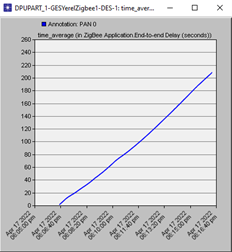
\includegraphics[width=5cm]{Resim/Sekil4-22.png}}


\centering
%ethernet haberleşmesinde LAN gecikme grafiğidir
\pgfplotsset{every axis/.append style={
font=\footnotesize,
thin,
tick style={ultra thin}},
scaled y ticks=false,
yticklabel style = {
/pgf/number format/fixed,
/pgf/number format/precision=5
},
}

    \begin{tikzpicture}
    \begin{axis}[
    xlabel={Simülasyon Süresi (Saniye)},
    ylabel={Uçtan Uca Gecikme (Saniye)},
    grid,
    legend style = {font=\tiny,at={(1,0.8)}, anchor=east}
    ]

\addplot [color=cyan, mark=star, mark repeat =14, mark size = 3]  table [x = Simulation Duration, y = GESYerelZigbee1EndtoendDelayseconds, col sep = comma] {fig4deneme (1).csv};
%\addlegendentry{Ethernet bağlantı gecikme değeri}



\end{axis}
\end{tikzpicture}

\caption{Yerel ağda yaşanan gecikme değişimi}
\label{fig:4-23}
\end{figure}

\begin{figure}[htbp]
%\centerline{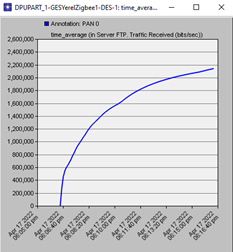
\includegraphics[width=5cm]{Resim/Sekil4-23.png}}

\centering
%ethernet haberleşmesinde LAN gecikme grafiğidir
\pgfplotsset{every axis/.append style={
font=\footnotesize,
thin,
tick style={ultra thin}},
scaled y ticks=false,
yticklabel style = {
/pgf/number format/fixed,
/pgf/number format/precision=5
},
}

    \begin{tikzpicture}
    \begin{axis}[
    xlabel={Simülasyon Süresi (Saniye)},
    ylabel={Yüklenen Veri Boyutu (Byte/s)},
    grid,
    legend style = {font=\tiny,at={(1,0.8)}, anchor=east}
    ]

\addplot [color=blue, mark=circle, mark repeat =14, mark size = 3]  table [x = Simulation Duration, y = GESYerelZigBeeApplicationTrafficReceivedbitssec, col sep = comma] {fig4deneme (1).csv};
%\addlegendentry{Ethernet bağlantı gecikme değeri}



\end{axis}
\end{tikzpicture}


\caption{Yerel ağdaki sunucuda toplanan veri boyutu}
\label{fig:4-24}
\end{figure}

\newpage
\paragraph{Rüzgar Enerji Sistemi}
Başlık \ref{zigbeeges112}'daki senaryonun \gls{res} versiyonu \gls{opnet} ortamında simülasyonu tamamlanmıştır. \gls{res}'dekine  ürettiği veri boyutu \gls{ges}'deki algılayı-cılardan fazladır. Bu sebeple Şekil \ref{fig:4-26}'deki veri boyutu Şekil \ref{fig:4-24}'daki yerel sunucuya yüklenen veri boyutundan fazladır. \gls{res}'deki ağ yapısında yaşanan gecikme değerleri Şekil \ref{fig:4-25}'de gösterilmiştir. İlgili gecikme değerleri \gls{iec} 61400 ve \gls{ieee} 1646 standartlarının belirlemiş olduğu gecikme değerlerine göre yüksektir. Bu durumda \gls{res}'deki enerji üretiminin gerçek zamanlı takibi yapılamamaktadır. 

\begin{figure}[htbp]
%\centerline{\includegraphics[width=5cm]{Resim/sekil4-24.png}}
\centering
%ethernet haberleşmesinde LAN gecikme grafiğidir
\pgfplotsset{every axis/.append style={
font=\footnotesize,
thin,
tick style={ultra thin}},
scaled y ticks=false,
yticklabel style = {
/pgf/number format/fixed,
/pgf/number format/precision=5
},
}

    \begin{tikzpicture}
    \begin{axis}[
    xlabel={Simülasyon Süresi (Saniye)},
    ylabel={Uçtan Uca Gecikme (Saniye)},
    grid,
    legend style = {font=\tiny,at={(1,0.8)}, anchor=east}
    ]

\addplot [color=cyan, mark=star, mark repeat =14, mark size = 3]  table [x = Simulation Duration, y = TurbinZigBeeApplicationEndtoendDelayseconds, col sep = comma] {fig4deneme (1).csv};
%\addlegendentry{Ethernet bağlantı gecikme değeri}



\end{axis}
\end{tikzpicture}


\caption{Yerel ağda yaşanan gecikme süresi}\label{fig:4-25}
\end{figure}

\begin{figure}[htbp]
%\centerline{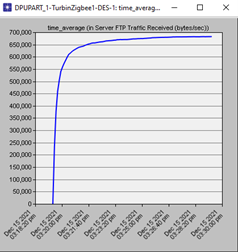
\includegraphics[width=5cm]{Resim/sekil4-25.png}}


\centering
%ethernet haberleşmesinde LAN gecikme grafiğidir
\pgfplotsset{every axis/.append style={
font=\footnotesize,
thin,
tick style={ultra thin}},
scaled y ticks=false,
yticklabel style = {
/pgf/number format/fixed,
/pgf/number format/precision=5
},
}

    \begin{tikzpicture}
    \begin{axis}[
    xlabel={Simülasyon Süresi (Saniye)},
    ylabel={Yüklenen Veri Boyutu (Byte/s)},
    grid,
    legend style = {font=\tiny,at={(1,0.8)}, anchor=east}
    ]

\addplot [color=blue, mark=circle, mark repeat =14, mark size = 3]  table [x = Simulation Duration, y = TurbinZigBeeApplicationTrafficReceived, col sep = comma] {fig4deneme (1).csv};
%\addlegendentry{Ethernet bağlantı gecikme değeri}



\end{axis}
\end{tikzpicture}

\caption{Yerel ağdaki sunucuda toplanan veri boyutu}
\label{fig:4-26}
\end{figure}


\newpage
\subsubsection{\gls{lan} tasarımı OPNET Simülasyon Sonuçları}


Zigbee, \gls{wifi} ve Ethernet altyapısında modellenen simülasyonların 2 \gls{myo}'daki sonuçları \ref{yerelEthernet}--\ref{zigbee} başlıklarında paylaşılmıştır. \gls{lan} simülasyon sonuçları incelendiğinde Zigbee altyapısı ile kurulan haberleşme trafiğinde gecikme değerleri ilgili standartların belirlemiş olduğu üst değer olan 1 saniyenin çok üzerindedir. Bu sebeple Geniş Alan Ağı tasarımının olduğu bölümde Zigbee altyapısı dahil edilmemiştir.

\section{OPNET GENİŞ ALAN AĞI TASARIM VE SİMÜLASYON SONUÇLARI}

Önceki bölümde \gls{lan} modeli incelenmiştir. Şekil \ref{fig:4-27}’de Google Earth yazılımında Kütahya’nın meslek yüksekokulları ve merkez kampüsü gösterilmiştir. Okullardaki enerji üretim sisteminin merkezi bir noktadan kontrolü gözlemi ve aksiyonu için \gls{iec}, veri haberleşmesinin en fazla 1 saniye gecikmesine izin vermiştir. Tasarım olarak enerji üretiminin izleme merkezi \gls{dpu} Merkez Kampüsü olarak belirlenmiştir. Geniş alan ağı tasarım senaryoları kablosuz ve kablolu olarak iki kısımda incelenmiştir.


\begin{figure}[htbp]
\centerline{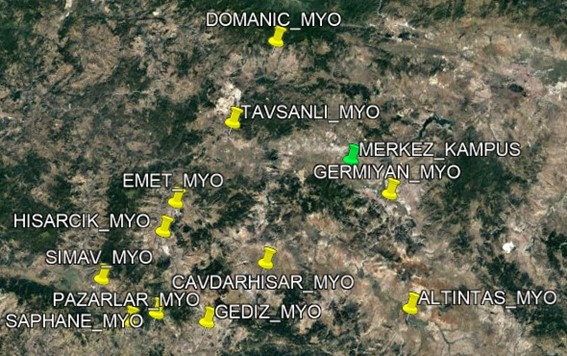
\includegraphics[width=10cm]{Resim/sekil4-26.jpg}}
\caption{\gls{dpu}’nün Meslek Yüksek Okulları ve Merkez Kampüsü}
\label{fig:4-27}
\end{figure}


\subsection{Kablosuz Geniş Ağ Tasarımı}

\ref{mikrohaberlesme} kısmında belirtilen kablosuz haberleşme tekniğinden \gls{wimax} teknolojisi kullanılarak meslek yüksekokulları arasında bir haberleşme linki kurulmuştur. Yüksek hızlarda haberleşme çözümü imkanı sağlayan \gls{wimax} teknolojisi 11-66 GHz arasında bir haberleşme taşıyıcı frekansına sahiptir. Bu frekans aralığındaki elektromanyetik dalganın boyu çok küçüktür. Elektromanyetik dalga için atmosfer soğurumu frekansın karesiyle ters orantılı olduğu için, yüksek frekans bölgesinde düşük kayıplı iletişim için doğrudan görüş hattında iletişim yapılması gereklidir.

İlgi \gls{myo}'ların \gls{dpu} merkez kampüsü ile sağlıklı bir haberleşme sağlaması için öncelikle sistemsel olarak Google Earth yazılımında Kütahya ilinin fiziki yükselti haritası incelenmiştir. Bu incelemelerin sonucunda 2 adet toplama noktası belirlenmiştir. Bu toplama noktaları ile üniversiteye ait kampüslerin birbirlerini doğrudan ve engelsiz bir şekilde görebildiği Google Earth yazılımından doğrulanmıştır.

Toplama noktalarıyla doğrudan haberleşen meslek yüksekokulları Tablo \ref{tab:tablo4-6}'da gösterilmiştir.



\begin{figure}[htbp]
\centerline{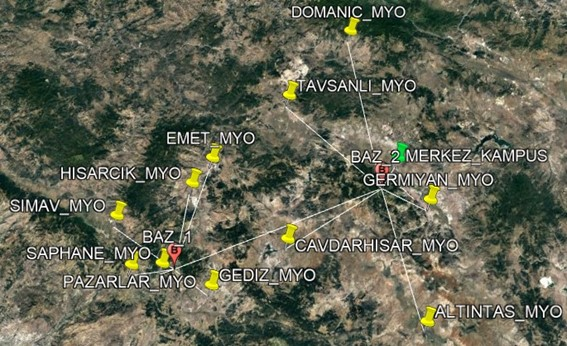
\includegraphics[width=10cm]{Resim/sekil4-27.jpg}}
\caption{Baz istasyonu vaziyet planı}
\label{fig:4-28}
\end{figure}




\begin{table}[htbp]
\centering
\caption{Yerleşkelerde kullanılan enerji sistemi ve bağlı olduğu baz istasyonları.}
\label{tab:tablo4-6}
\begin{tabular}{|l|c|l|c|}
\hline
Yerleşke İsmi        & \multicolumn{1}{l|}{Baz No} & Yerleşke İsmi         & \multicolumn{1}{l|}{Baz No} \\ \hline
Pazarlar \gls{myo} (Güneş) & \multirow{6}{*}{1}          & Tavşanlı \gls{myo} (Rüzgar) & \multirow{6}{*}{2}          \\ \cline{1-1} \cline{3-3}
Hisarcık \gls{myo} (Rüzgar) &  & Domanic \gls{myo} (Rüzgar)    &  \\ \cline{1-1} \cline{3-3}
Şaphane \gls{myo} (Güneş)   &  & Germiyan \gls{myo} (Rüzgar)   &  \\ \cline{1-1} \cline{3-3}
Gediz \gls{myo} (Güneş)     &  & Altıntaş \gls{myo} (Güneş)    &  \\ \cline{1-1} \cline{3-3}
Simav \gls{myo} (Rüzgar)    &  & Çavdarhisar \gls{myo} (Güneş) &  \\ \cline{1-1} \cline{3-3}
Emet \gls{myo} (Rüzgar)     &  & Merkez Kampüs (İzleme)  &  \\ \hline
\end{tabular}
\end{table}


\begin{figure}[htbp]
\centerline{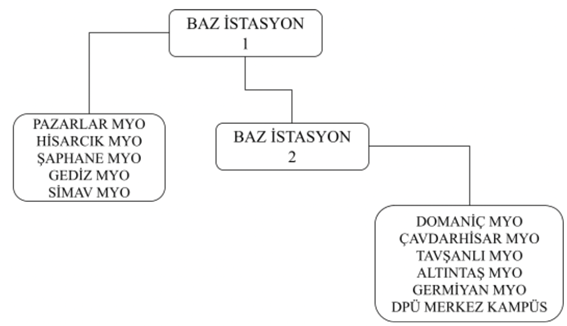
\includegraphics[width=10cm]{Resim/sekil4-28.png}}
\caption{Baz istasyonları bağlantı topolojisi}
\label{fig:4-29}
\end{figure}

\gls{wimax} haberleşmesinde minimum veri kullanımı önemli bir faktördür. Gereksiz veri trafiği en istenmeyen durumdur. Bölüm \ref{motivasyon}'de belirtildiği üzere amaçlanan kriter minimum haberleşme maliyeti ile maksimum performansta bir haberleşme çözümü sunmaktır. Bu nedenle lokal bölgelerde oluşturulan verilerin \gls{dpu} Merkez kampüsüne ileti-lirken diğer lokal bölgelere iletilmesinin önüne geçilmelidir. 

Günümüzde IP haberleşmesinde farklı ağları birbirleriyle haberleştirme tekniği olarak yönlendirme protokolleri kullanılmaktadır. 
Kullanıcı kendi yerel alan ağı dışındaki bir noktaya veri gönderebilmek için yerel ağındaki yönlendiriciye verisini iletir; yönlendirici de nihai hedefe doğru verileri iletir. Nihai hedefin yerel alan ağından sorumlu yönlendiriciye kadar belirli cihazlar arasında atlama yapmaktadır. Uçtan uca yol boyunca her yönlendirici, hedefe ulaşmak için kullanılan bir sonraki atlama cihazını seçer. Sonraki atlama, hedefe ulaşmak için yol boyunca bir sonraki cihazı temsil eder. Böylelikle rotalama tekniği uygulanmış olur. 

IP yönlendirme metodu statik ve dinamik olarak iki kısımda incelenir. Bu tezde veri trafiklerini geniş alan ağlarında yönetmek için statik yönlendirme kullanılmıştır.

Statik yönlendirme, ağ yöneticisi tarafından tasarlanır ve ağa uygulanır. Ağ yöneticisinin sorumluluğunda bütün trafik şekillenmektedir. Statik yönlendirmenin tercih edilme sebepleri aşağıda paylaşılmıştır. \cite{parziale_2006}

•	Yönlendirme algoritmasına göre daha spesifik bir rota içermediğinde trafiği iletmek için tercih edilir.

•	Karmaşık yönlendirme ilkeleri gerektiğinde kullanılır. Örnek olarak, belirli bir ana bilgisayara yönlendirilen trafiğin belirlenmiş bir ağ yolundan geçmesini garanti etmek gibi bir senaryo gerektiğinde statik yönlendirme tekniği kullanılır.

•	Ağ yöneticisi, kurulu sistemde tanımlanan tüm ağların sınıfı veya özelliğine göre birbirleriyle spesifik verilerin haberleşmesini sağlamak için statik yönlendirme kullanmaktadır. 

•	Statik yönlendirme yöntemi, komşu cihazlar arasında rota bilgilerini tanıtmayı gerektirmez. Bu durum sayesinde haberleşmede kullanılan bant genişliğinden tasarruf edilir. Ayrıca, ağ yollarını hesaplamak için daha az işlemci önbelleği ve döngüsü kullanılır.

\gls{wimax} teknolojisinde veri trafiğinde kullanılan bant genişliği çok önemli bir konudur. Bilindiği üzere \gls{wimax} lisanslı bir bant üzerinden haberleşmesini yapmaktadır, yani limitli bir bant genişliği kullanımı söz konusudur. Bu nedenle yerel noktalarda oluşturulan verilerin en az bant genişliği kullanılarak gönderilmesi amaçlanmıştır. Statik yönlendirme tekniği de bu sebepten kullanılmaktadır. Bu teknik sayesinde aynı baz istasyonlarına bağlı farklı meslek yüksekokulları, birbirlerinin haberleşme bant genişliğini işgal etmemektedir. Merkez noktadaki toplama noktasına gönderilen veriler böylelikle korunmuş olur ayrıca başka noktalarda gereksiz veri boyutu kullanımının önüne geçilmiş olur.

\begin{figure}[htbp]
\centerline{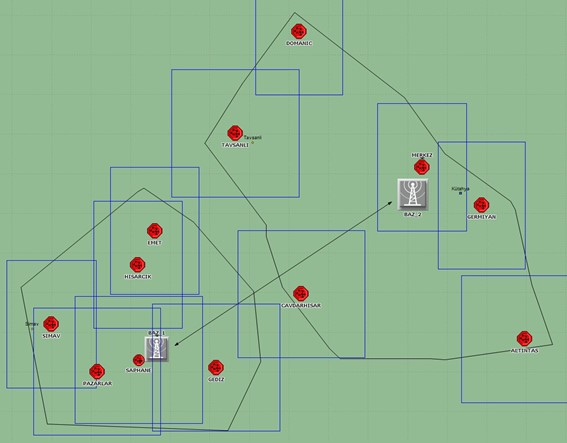
\includegraphics[width=\columnwidth]{Resim/sekil4-29.jpg}}
\caption{OPNET ortamında tasarlanan WAN yerleşim planında iki adet baz istasyonu bulunmaktadır. Baz istasyonlarının kapsama alanları gösterilmiştir. \gls{myo}'larda üretilen tüm veriler baz istasyonları aracılığıyla merkez'e iletilmektedir.}
\label{fig:4-30}
\end{figure}



\subsubsection{Senaryo:1}\label{senaryo1}

\gls{wimax} teknolojisi ile haberleşilen geniş alan ağının ilk senaryosunda \gls{wimax} altyapısı kullanılmıştır. Meslek Yüksekokullarında üretilen algılayıcı verileri \gls{wifi} altyapısında haberleşmektedir. Yapılan senaryo tasarımı sonrasında tüm \gls{myo}'larda bulunan algılayıcı düğümlerinde gözlemlenen ortalama gecikme (delay) değeri 0.06 saniye değerindedir. Gecikme değeri, aynı haberleşme protokolünde çalışan iki düğüm arasında paket gönderim süresi olarak tanımlanmıştır. Şekil \ref{fig:4-31}’de gözlemlenen gecikme değişimi \gls{iec} 61400 ve \gls{iec} 61724 standartlarını karşılamaktadır. 12 adet kampüs içi yerel alan ağının \gls{wifi} üzerinden haberleşme yapılması durumuyla birleştirilmiş \gls{wimax} geniş alan ağı teknolojisinde yaşanan gecikmenin grafiği Şekil \ref{fig:4-31}’de paylaşılmıştır.



\begin{figure}[htbp]
%\centerline{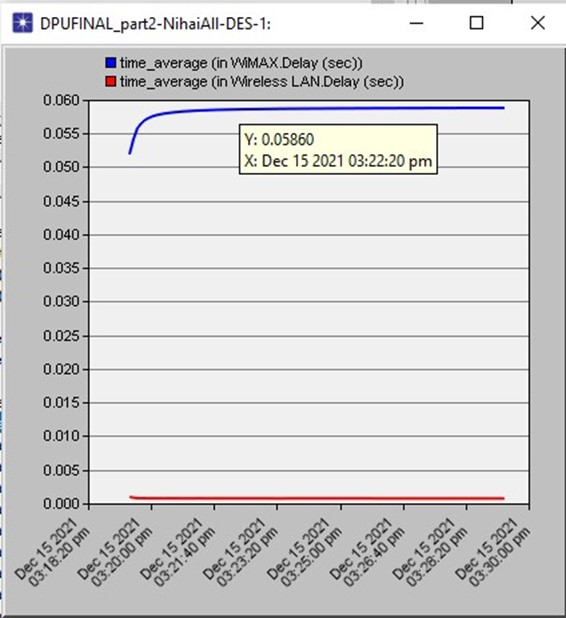
\includegraphics[width=10cm]{Resim/Sekil4-30.jpg}}

\centering
\pgfplotsset{every axis/.append style={
font=\footnotesize,
thin,
tick style={ultra thin}},
}
    \begin{tikzpicture}
\begin{semilogyaxis}[ymax = 0.070000,
xlabel={Simülasyon Süresi (Saniye)},
ylabel={Gecikme Süresi (Saniye)},
xmode=normal, ymode=log, 
grid = major,
log ticks with fixed point,
ytick={0.05,0.0005, 0.01,0.001,0.0001,0.005},
legend style = {font=\tiny,at={(1,0.3)}, anchor=east}
]


\addplot [color=blue, mark=oplus*, mark repeat =14, mark size = 3]  table [x = Simulation Duration, y = Senaryo1WimaxDelay, col sep = comma] {fig4deneme (1).csv};


%--
\addplot [color=red, mark=pentagon*, mark repeat =14, mark size = 3, mark phase = 8]  table [y = Senaryo1WifiDelay, col sep = comma] {fig4deneme (1).csv};

%--

\legend{Wimax Gecikme, WiFi Gecikme }
\end{semilogyaxis}



\end{tikzpicture}


\caption{\gls{wimax} ve \gls{wifi} teknolojisinde gözlemlenen gecikme değeri}
\label{fig:4-31}
\end{figure}

\gls{dpu} merkez kampüsünde kurulan ana sunucuya gönderilen toplam veri boyutunun anlık grafiği Şekil \ref{fig:4-32}’de gösterilmiştir. Kurulu olan güneş ve rüzgar enerji sistemlerinde üretilen verilerin toplam boyutu, ana sunucuya gelen veri boyutuyla aynıdır. Şekil \ref{fig:4-32}'e bakarak 11 adet \gls{myo}'da bir veri kaybının olmadığı görülmektedir.

\begin{figure}[htbp]
%\centerline{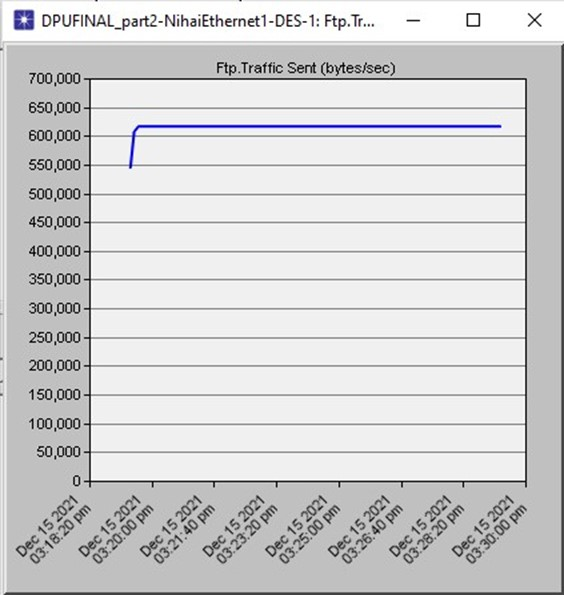
\includegraphics[width=10cm]{Resim/Sekil4-31.jpg}}
\centering
%ethernet haberleşmesinde LAN gecikme grafiğidir
\pgfplotsset{every axis/.append style={
font=\footnotesize,
thin,
tick style={ultra thin}},
scaled y ticks=false,
yticklabel style = {
/pgf/number format/fixed,
/pgf/number format/precision=5
},
}

    \begin{tikzpicture}
    \begin{axis}[ymax = 700000.0000000,
    xlabel={Simülasyon süresi (Saniye)},
    ylabel={Yüklenen Veri Boyutu (Byte/s)},
    grid,
    legend style = {font=\tiny,at={(1,0.8)}, anchor=east}
    ]

\addplot [color=blue, mark=circle, mark repeat =14, mark size = 3]  table [x = Simulation Duration, y = TOTALReceivedAllScenario, col sep = comma] {fig4deneme (1).csv};
%\addlegendentry{Ethernet bağlantı gecikme değeri}



\end{axis}
\end{tikzpicture}


\caption{Ana sunucuda toplanan verilerin değeri}
\label{fig:4-32}
\end{figure}


Simülasyon sonucunda ana sunucuya gelen algılayıcıların anlık veri boyutları Resim \ref{fig:4-33}’te gösterilmiştir. Örneğin, Tablo \ref{tab:tablo4-5}’teki rüzgar algılayıcılarının ürettikleri veri değeri 6 Byte/s değerindedir, bu durum ile birlikte Tablo \ref{tab:tablo4-4}’teki rüzgar enerji türbininin rotor modülü 12010 Byte/s değerinde veri üretmektedir. İlgili \gls{wan} senaryosunda 5 adet \gls{ges}, 5 adet \gls{res} bulunmaktadır. Simülasyon sonucunda "Rüzgar Hızı" algılayıcıları toplamda 30 Byte/s'lik, "WROT" algılayıcıları toplamda 72.060 Byte/s'lik hızlarda ana sunucuya veri göndermişlerdir. Farklı algılayıcının üretmiş olduğu veri miktarlarının aynı grafikte birlikte gösterilebilmesi için logaritmik eksen tercih edilmiştir. 
%bunu tablo olarak göster


\begin{comment}

\begin{table}[htbp]
\centering
\caption{Ana sunucada toplanan algılayıcılarıcıların anlık değişimi}
\label{fig:4-33}
\begin{tabular}{cc}
\hline
\begin{tabular}[c]{@{}c@{}}Algılayıcı\\ Tanımı\end{tabular} & \begin{tabular}[c]{@{}c@{}}Merkez Sunucuya\\ İletilen Veri \end{tabular} \\ \hline
Meteoroloji         & 50 B/s         \\
İnverter Akım       & 72.000 B/s         \\
İnverter Gerilim    & 72.000 B/s         \\
Rüzgar Hızı         & 30 B/s    \\
Radyant Işıma       & 1.000 B/s    \\
WCNV                & 75.020 B/s         \\
WGEN                & 70.020 B/s         \\
WMET                & 40.000 B/s    \\
WNAC                & 66.048 B/s    \\
WROT                & 60.050 B/s       \\
WTOW                & 12.036 B/s       \\
WTRF                & 48.036 B/s       \\
WTRM                & 72.096 B/s       \\
WYAW                & 36.024 B/s       \\
WROT                & 60.050 B/s       \\ \hline
TOTAL & 684.460 B/s       \\ \hline
\end{tabular}
\end{table}
\end{comment}




\begin{figure}[htbp]
%\centerline{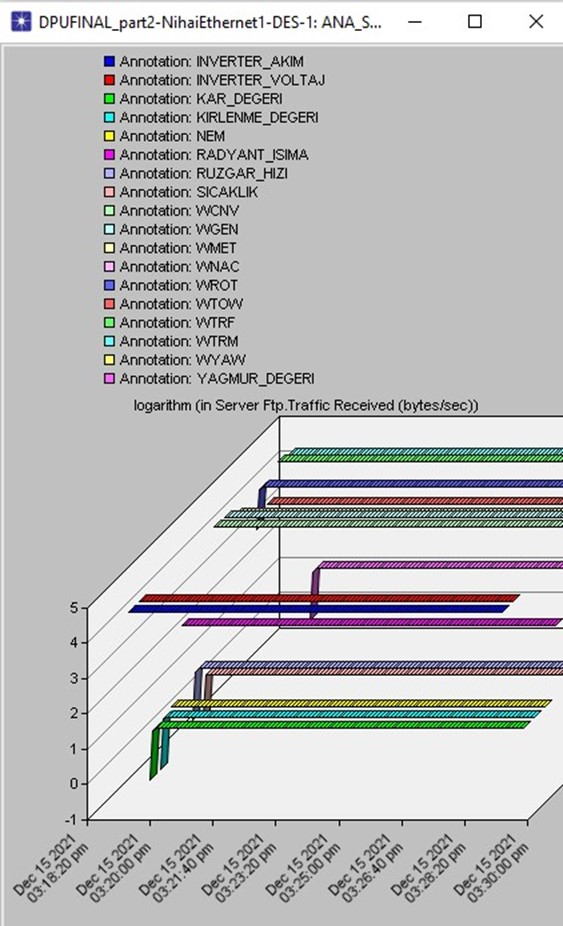
\includegraphics[width=10cm]{Resim/Sekil4-32.jpg}}

\centering
\pgfplotsset{every axis/.append style={
font=\footnotesize,
thin,
tick style={ultra thin}},
scaled y ticks=false,
yticklabel style = {
/pgf/number format/fixed,
/pgf/number format/precision=5
},
}
    \begin{tikzpicture}
\begin{semilogyaxis}[
zmode = log,
zmin = 1,
xlabel={Simülasyon Süresi (Saniye)},
zlabel={Yüklenen Veri Boyutu (Byte/s)},
ytick = \empty,
grid = major,
log ticks with fixed point,
legend style = {font=\tiny,at={(1,0.8)}, anchor=east},
area plot1/.style={%ilk alan için oluşturulan saydanlık vs.
fill opacity=0.33,
draw = orange!80!black,thick,
fill = orange,
mark=none,
},
area plot2/.style={
fill opacity=0.33,
draw = blue!80!black,thick,
fill = blue,
mark=none,
},
area plot3/.style={
fill opacity=0.33,
draw = cyan!80!black,thick,
fill = cyan,
mark=none,
},
area plot4/.style={
fill opacity=0.33,
draw = red!80!black,thick,
fill = red,
mark=none,
},
area plot5/.style={
fill opacity=0.33,
draw = yellow!80!black,thick,
fill = yellow,
mark=none,
},
area plot6/.style={
fill opacity=0.23,
draw = gray!80!black,thick,
fill = gray,
mark=none,
},
area plot7/.style={
fill opacity=0.23,
draw = purple!80!black,thick,
fill = purple,
mark=none,
},
area plot8/.style={
fill opacity=0.23,
draw = green!80!black,thick,
fill = green,
mark=none,
},
legend pos = outer north east,]
%bu kısımda turbinlerin hepsini plot3'e ekliyoruz
\addplot3+ [area plot1]  table [x = Simulation Duration, y = eksen1, z = TrafficReceivedbytessecINVERTERAKIM, col sep = comma] {fig4deneme (1).csv} \closedcycle;
\addlegendentry{İnverter Akım}
%---------

\addplot3+ [area plot1]  table [y = eksen2, z = TrafficReceivedbytessecINVERTERVOLTAJ, col sep = comma] {fig4deneme (1).csv} \closedcycle;
\addlegendentry{İnverter Gerilim}
%---------

\addplot3+ [area plot2]  table [y = eksen3, z = TrafficReceivedbytessecMETEOR, col sep = comma] {fig4deneme (1).csv} \closedcycle;
\addlegendentry{Meteoroloji}
%---------


\addplot3+ [area plot3]  table [y = eksen4, z = TrafficReceivedbytessecRADYANTISIMA, col sep = comma] {fig4deneme (1).csv} \closedcycle;
\addlegendentry{Radyant Işıma}
%---------


\addplot3+ [area plot4]  table [y = eksen5, z = TrafficReceivedbytessecRUZGARHIZI, col sep = comma] {fig4deneme (1).csv} \closedcycle;
\addlegendentry{Rüzgar Hızı}
%---------


\addplot3+ [area plot5]  table [y = eksen6, z = TrafficReceivedbytessecWCNV, col sep = comma] {fig4deneme (1).csv} \closedcycle;
\addlegendentry{WCNV}
%---------

\addplot3+ [area plot6]  table [y = eksen7, z = TrafficReceivedbytessecWGEN, col sep = comma] {fig4deneme (1).csv} \closedcycle;
\addlegendentry{WCNV}
%---------

\addplot3+ [area plot7]  table [y = eksen8, z = TrafficReceivedbytessecWMET, col sep = comma] {fig4deneme (1).csv} \closedcycle;
\addlegendentry{WMET}
%---------


\addplot3+ [area plot2]  table [y = eksen9, z = TrafficReceivedbytessecWNAC, col sep = comma] {fig4deneme (1).csv} \closedcycle;
\addlegendentry{WNAC}
%---------

\addplot3+ [area plot1]  table [y = eksen10, z = TrafficReceivedbytessecWROT, col sep = comma] {fig4deneme (1).csv} \closedcycle;
\addlegendentry{WROT}
%---------


\addplot3+ [area plot3]  table [y = eksen11, z = TrafficReceivedbytessecWTOW, col sep = comma] {fig4deneme (1).csv} \closedcycle;
\addlegendentry{WTOW}
%---------

\addplot3+ [area plot4]  table [y = eksen12, z = TrafficReceivedbytessecWTRF, col sep = comma] {fig4deneme (1).csv} \closedcycle;
\addlegendentry{WTRF}
%---------


\addplot3+ [area plot2]  table [y = eksen13, z = TrafficReceivedbytessecWTRM, col sep = comma] {fig4deneme (1).csv} \closedcycle;
\addlegendentry{WTRM}
%---------

\addplot3+ [area plot2]  table [y = eksen14, z = TrafficReceivedbytessecWYAW, col sep = comma] {fig4deneme (1).csv} \closedcycle;
\addlegendentry{WYAW}
%---------


\end{semilogyaxis}
\end{tikzpicture}


\caption{Ana sunuca toplanan algılayıcı düğümlerin logaritmik değeri}
\label{fig:4-33}
\end{figure}


Tablo \ref{tab:tablo4-6}’ya göre \gls{myo}'larda üretilen algılayıcı verilerinin \gls{dpu} komuta merkezi sunucusuna gönderilme zamanı Şekil \ref{fig:4-34}’de gösterilmiştir. Bu grafiğe göre üretilen veriler yaklaşık 0.46 saniyelik gecikme ile ana sunucuda toplandığı gözlemlenmiştir. Geniş alan ağında, \gls{iec} standartlarına göre, verilerin 1 saniyenin altında bir süre ile hedef noktasına iletilmesi gerektiği belirtilmektedir \cite{mackiewicz2006overview}. Buna göre tasarlanan \gls{wifi} ve \gls{wimax} hibrit teknolojili haberleşme ağı ilgili standartları tamamen karşılamaktadır

\begin{figure}[htbp]
%\centerline{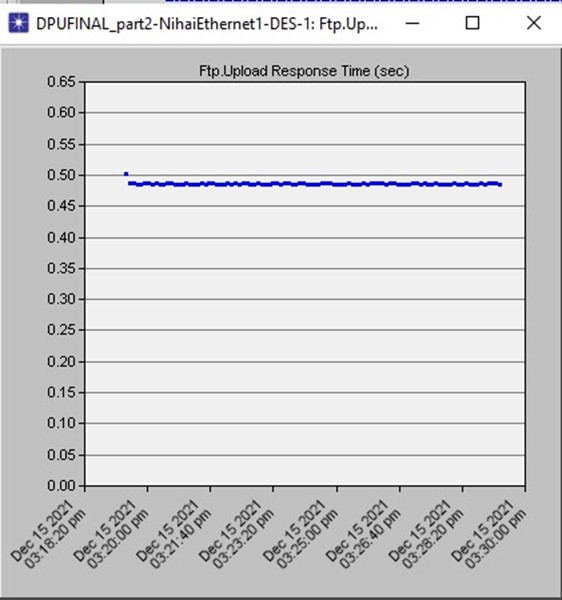
\includegraphics[width=10cm]{Resim/Sekil4-33.jpg}}
\centering
%ethernet haberleşmesinde LAN gecikme grafiğidir
\pgfplotsset{every axis/.append style={
font=\footnotesize,
thin,
tick style={ultra thin}},
scaled y ticks=false,
yticklabel style = {
/pgf/number format/fixed,
/pgf/number format/precision=5
},
}

    \begin{tikzpicture}
    \begin{axis}[
    xlabel={Simülasyon süresi (Saniye)},
    ylabel={Veri Yükleme Süresi (Saniye)},
    grid,
    legend style = {font=\tiny,at={(1,0.8)}, anchor=east}
    ]

\addplot [color=blue, mark=circle, mark repeat =14, mark size = 3]  table [x = Simulation Duration, y = Senaryo1uploadResponseTime, col sep = comma] {fig4deneme (1).csv};
%\addlegendentry{Ethernet bağlantı gecikme değeri}



\end{axis}
\end{tikzpicture}


\caption{Enerji sistemlerindeki algılayıcı verilerin ana sunucuya ortalama ulaşma süresi}
\label{fig:4-34}
\end{figure}
\newpage
\subsubsection{Senaryo:2}\label{senaryo2}

11 adet \gls{myo}'da kurulmuş olan UTP altyapılı haberleşme sisteminde gözlemlenen ortalama gecikme değeri Şekil \ref{fig:4-35}’te görüldüğü üzere yaklaşık 0.00015 saniyedir. İlgili MYO'ların \gls{wimax} altyapısındaki ortalama gecikme değeri 0.06 saniye değerindedir. 
Bu değerler, yerel alan ağında \gls{wifi} teknolojisi kullanıldığı duruma göre daha iyidir. 

\begin{figure}[htbp]
%\centerline{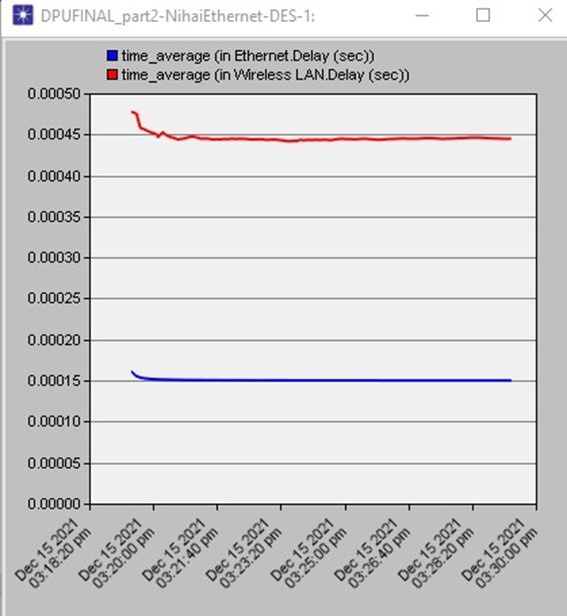
\includegraphics[width=10cm]{Resim/Sekil4-34.jpg}}

\centering
\pgfplotsset{every axis/.append style={
font=\footnotesize,
thin,
tick style={ultra thin}},
}
    \begin{tikzpicture}
\begin{semilogyaxis}[ymax = 0.070000,
xlabel={Simülasyon Süresi (Saniye)},
ylabel={Gecikme Süresi (Saniye)},
xmode=normal, ymode=log, 
grid = major,
log ticks with fixed point,
ytick={0.05,0.0005, 0.01,0.001,0.0001,0.005},
legend style = {font=\tiny,at={(1,0.3)}, anchor=east}
]


\addplot [color=blue, mark=oplus*, mark repeat =14, mark size = 3]  table [x = Simulation Duration, y = Senaryo2WimaxDelay, col sep = comma] {fig4deneme (1).csv};


%--
\addplot [color=red, mark=pentagon*, mark repeat =14, mark size = 3, mark phase = 8]  table [y = Senaryo2UTPEthernet Delay, col sep = comma] {fig4deneme (1).csv};

%--

\legend{Wimax Gecikme, WiFi Gecikme }
\end{semilogyaxis}



\end{tikzpicture}



\caption{\gls{wimax} ve Ethernet teknolojisinde gözlemlenen gecikme değeri}
\label{fig:4-35}
\end{figure}

Şekil \ref{fig:4-36}’de \gls{dpu}’nün merkez kampüsünde kurulan ana sunucuya gönderilen toplam verinin değişim grafiğine bakıldığında, bölüm \ref{senaryo1} Şekil \ref{fig:4-32}'deki performans değerleriyle neredeyse aynı olduğu görülmüştür. 


\begin{figure}[htbp]
%\centerline{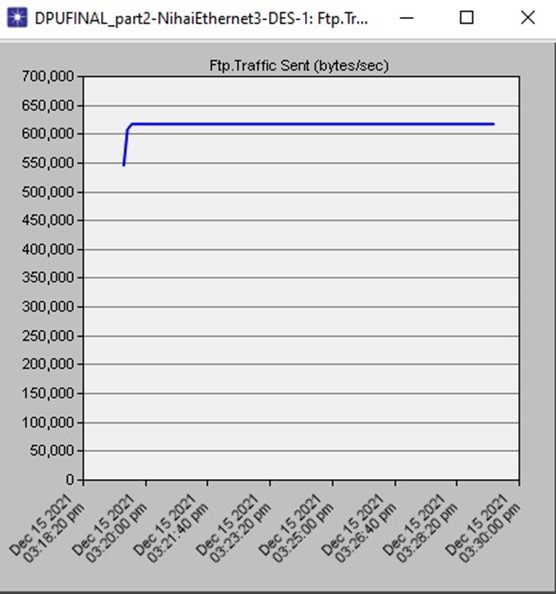
\includegraphics[width=10cm]{Resim/Sekil4-35.jpg}}


\centering
%ethernet haberleşmesinde LAN gecikme grafiğidir
\pgfplotsset{every axis/.append style={
font=\footnotesize,
thin,
tick style={ultra thin}},
scaled y ticks=false,
yticklabel style = {
/pgf/number format/fixed,
/pgf/number format/precision=5
},
}

    \begin{tikzpicture}
    \begin{axis}[ymax = 700000,
    xlabel={Simülasyon süresi (Saniye)},
    ylabel={Yüklenen Veri Boyutu (Byte/s)},
    grid,
    legend style = {font=\tiny,at={(1,0.8)}, anchor=east}
    ]

\addplot [color=red, mark=circle, mark repeat =14, mark size = 3]  table [x = Simulation Duration, y = TOTALReceivedAllScenario, col sep = comma] {fig4deneme (1).csv};
%\addlegendentry{Ethernet bağlantı gecikme değeri}



\end{axis}
\end{tikzpicture}


\caption{Ana sunucuda toplanan verilerin boyutu}
\label{fig:4-36}
\end{figure}


Ana sunucuda toplanan algılayıcı modüllerin anlık değeri Şekil \ref{fig:4-37}’de görülmektedir. Yerel ağda \gls{wifi} teknolojisi kullanıldığında da aynı değerler elde edilmiştir. Buna göre haberleşme trafiğinde yerel ağ teknolojisinin Ethernet veya \gls{wifi} olması veri aktarımında bir performans değişikliği oluşturmamaktadır.

\begin{figure}[htbp]
%\centerline{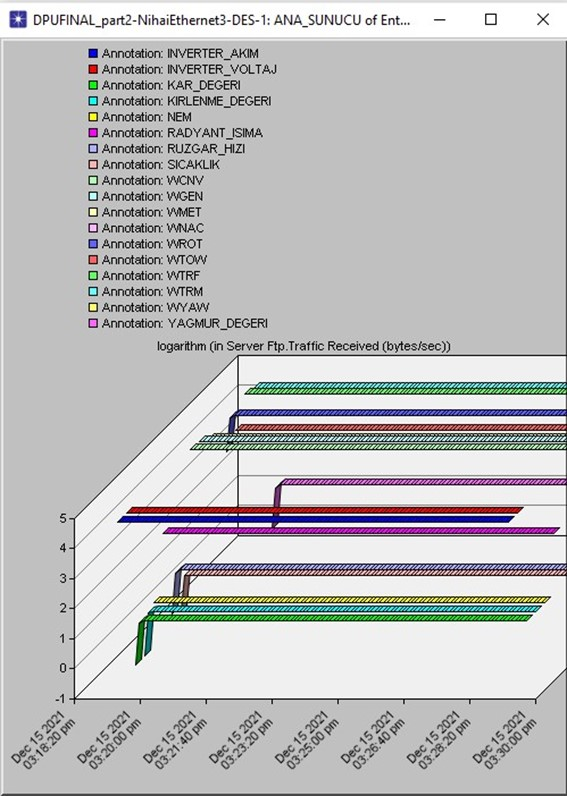
\includegraphics[width=10cm]{Resim/sekil4-36.jpg}}



\centering
\pgfplotsset{every axis/.append style={
font=\footnotesize,
thin,
tick style={ultra thin}},
scaled y ticks=false,
yticklabel style = {
/pgf/number format/fixed,
/pgf/number format/precision=5
},
}
    \begin{tikzpicture}
\begin{semilogyaxis}[
zmode = log,
zmin = 1,
xlabel={Simülasyon Süresi (Saniye)},
zlabel={Yüklenen Veri Boyutu (Byte/s)},
ytick = \empty,
grid = major,
log ticks with fixed point,
legend style = {font=\tiny,at={(1,0.8)}, anchor=east},
area plot1/.style={%ilk alan için oluşturulan saydanlık vs.
fill opacity=0.33,
draw = orange!80!black,thick,
fill = orange,
mark=none,
},
area plot2/.style={
fill opacity=0.33,
draw = blue!80!black,thick,
fill = blue,
mark=none,
},
area plot3/.style={
fill opacity=0.33,
draw = cyan!80!black,thick,
fill = cyan,
mark=none,
},
area plot4/.style={
fill opacity=0.33,
draw = red!80!black,thick,
fill = red,
mark=none,
},
area plot5/.style={
fill opacity=0.33,
draw = yellow!80!black,thick,
fill = yellow,
mark=none,
},
area plot6/.style={
fill opacity=0.23,
draw = gray!80!black,thick,
fill = gray,
mark=none,
},
area plot7/.style={
fill opacity=0.23,
draw = purple!80!black,thick,
fill = purple,
mark=none,
},
area plot8/.style={
fill opacity=0.23,
draw = green!80!black,thick,
fill = green,
mark=none,
},
legend pos = outer north east,]
%bu kısımda turbinlerin hepsini plot3'e ekliyoruz
\addplot3+ [area plot1]  table [x = Simulation Duration, y = eksen1, z = TrafficReceivedbytessecINVERTERAKIM, col sep = comma] {fig4deneme (1).csv} \closedcycle;
\addlegendentry{İnverter Akım}
%---------

\addplot3+ [area plot1]  table [y = eksen2, z = TrafficReceivedbytessecINVERTERVOLTAJ, col sep = comma] {fig4deneme (1).csv} \closedcycle;
\addlegendentry{İnverter Gerilim}
%---------

\addplot3+ [area plot2]  table [y = eksen3, z = TrafficReceivedbytessecMETEOR, col sep = comma] {fig4deneme (1).csv} \closedcycle;
\addlegendentry{Meteoroloji}
%---------


\addplot3+ [area plot1]  table [y = eksen4, z = TrafficReceivedbytessecRADYANTISIMA, col sep = comma] {fig4deneme (1).csv} \closedcycle;
\addlegendentry{Radyant Işıma}
%---------


\addplot3+ [area plot2]  table [y = eksen5, z = TrafficReceivedbytessecRUZGARHIZI, col sep = comma] {fig4deneme (1).csv} \closedcycle;
\addlegendentry{Rüzgar Hızı}
%---------


\addplot3+ [area plot5]  table [y = eksen6, z = TrafficReceivedbytessecWCNV, col sep = comma] {fig4deneme (1).csv} \closedcycle;
\addlegendentry{WCNV}
%---------

\addplot3+ [area plot6]  table [y = eksen7, z = TrafficReceivedbytessecWGEN, col sep = comma] {fig4deneme (1).csv} \closedcycle;
\addlegendentry{WCNV}
%---------

\addplot3+ [area plot7]  table [y = eksen8, z = TrafficReceivedbytessecWMET, col sep = comma] {fig4deneme (1).csv} \closedcycle;
\addlegendentry{WMET}
%---------


\addplot3+ [area plot2]  table [y = eksen9, z = TrafficReceivedbytessecWNAC, col sep = comma] {fig4deneme (1).csv} \closedcycle;
\addlegendentry{WNAC}
%---------

\addplot3+ [area plot1]  table [y = eksen10, z = TrafficReceivedbytessecWROT, col sep = comma] {fig4deneme (1).csv} \closedcycle;
\addlegendentry{WROT}
%---------


\addplot3+ [area plot3]  table [y = eksen11, z = TrafficReceivedbytessecWTOW, col sep = comma] {fig4deneme (1).csv} \closedcycle;
\addlegendentry{WTOW}
%---------

\addplot3+ [area plot4]  table [y = eksen12, z = TrafficReceivedbytessecWTRF, col sep = comma] {fig4deneme (1).csv} \closedcycle;
\addlegendentry{WTRF}
%---------


\addplot3+ [area plot2]  table [y = eksen13, z = TrafficReceivedbytessecWTRM, col sep = comma] {fig4deneme (1).csv} \closedcycle;
\addlegendentry{WTRM}
%---------

\addplot3+ [area plot7]  table [y = eksen14, z = TrafficReceivedbytessecWYAW, col sep = comma] {fig4deneme (1).csv} \closedcycle;
\addlegendentry{WYAW}
%---------


\end{semilogyaxis}
\end{tikzpicture}

\caption{Ana sunuca toplanan algılayıcıların veri değişimi}
\label{fig:4-37}
\end{figure}

Tablo \ref{tab:tablo4-6}’ya göre meslek yüksek okullarında üretilen algılayıcı verilerinin \gls{dpu} \\komuta merkezi sunucusuna gönderilme zamanı Şekil \ref{fig:4-38}’de gösterilmiştir. Bu grafiğe göre üretilen veriler yaklaşık 0.41 saniyelik gecikme ile ana sunucuda toplandığı gözlemlenir. Geniş ağ teknolojisindeki \gls{iec} standartlarında verilerin 1 saniyenin altında bir süre ile hedef noktasına iletilmesi gerektiği belirtilmektedir \cite{mackiewicz2006overview}. Buna göre tasarlanan Ethernet ve \gls{wimax} hibrit teknolojili haberleşme sistemi ilgili standartları tamamen karşılamaktadır.


\begin{figure}[htbp]
%\centerline{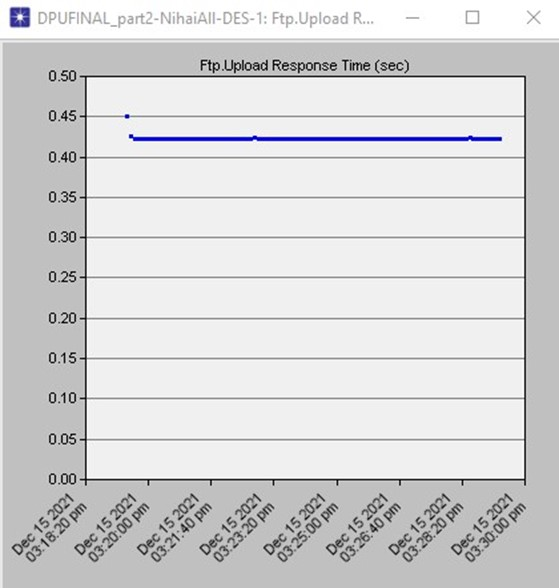
\includegraphics[width=10cm]{Resim/sekil4-37.jpg}}
\centering
%ethernet haberleşmesinde LAN gecikme grafiğidir
\pgfplotsset{every axis/.append style={
font=\footnotesize,
thin,
tick style={ultra thin}},
scaled y ticks=false,
yticklabel style = {
/pgf/number format/fixed,
/pgf/number format/precision=5
},
}

    \begin{tikzpicture}
    \begin{axis}[
    xlabel={Simülasyon süresi (Saniye)},
    ylabel={Veri Yükleme Süresi (Saniye)},
    grid,
    legend style = {font=\tiny,at={(1,0.8)}, anchor=east}
    ]

\addplot [color=blue, mark=circle, mark repeat =14, mark size = 3]  table [x = Simulation Duration, y = Senaryo2uploadResponseTime, col sep = comma] {fig4deneme (1).csv};
%\addlegendentry{Ethernet bağlantı gecikme değeri}



\end{axis}
\end{tikzpicture}


\caption{Upload Response Time}
\label{fig:4-38}
\end{figure}

\newpage
\subsection{Fiber Altyapılı Geniş Ağ Tasarımı}\label{fibeeraciklama}


Yerel internet sağlayıcıları üzerinden tarife anlaşması sağlanarak kurulmaktadır. Fakat telekom hattı sadece \gls{dpu} hizmet vermemekle birlikte hizmet sağladığı noktalardaki başka aboneleriyle birlikte ortak bir haberleşme havuzundan haberleşme hizmeti vermektedir. Bu hizmetin finansal açıdan ilk başta avantajının olması kaçınılmazdır. Fakat üniversiteye bağlı \gls{myo}'ların haberleşme güvenliğinin sağlanması son kullanıcının sorumluluğunda olacaktır. Buna göre ilgili meslek yüksekokullarına kurulacak harici bir güvenlik duvarı ve yönlendirici donanımlarıyla yerel ağlarda toplanan algılayıcı verileri fiziki bir güvenlik duvarından geçerek yönlendiriciler üzerinden \gls{dpu} Merkez kampüsüne ulaşır.


\begin{figure}[htbp]
\centerline{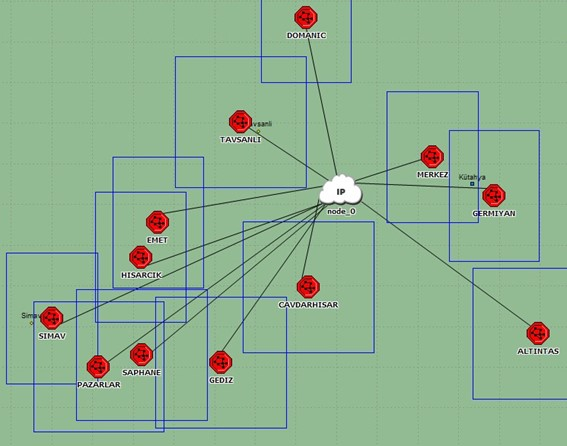
\includegraphics[width=10cm]{Resim/sekil4-39.jpg}}
\caption{Telekom altyapısına ait fiber optik ağın, önerilen dağıtık algılayıcı haberleşme ağına uyarlanması}
\label{fig:4-39}
\end{figure}

Şekil \ref{fig:4-40}’da görüldüğü üzere ana sunucuya iletilen verilerin süresi paylaşılır. Verilerin fiber optik altyapıyla iletilmesi, veri hızı açısından en etkili yöntemdir.

\begin{figure}[htbp]
%\centerline{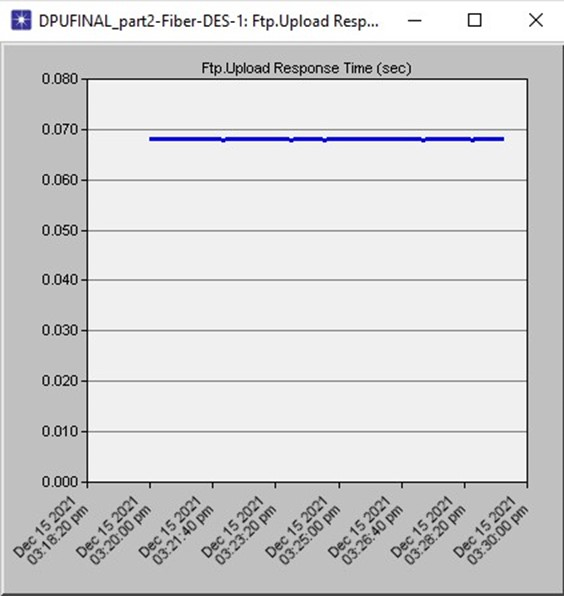
\includegraphics[width=10cm]{Resim/sekil4-38.jpg}}
\centering
%ethernet haberleşmesinde LAN gecikme grafiğidir
\pgfplotsset{every axis/.append style={
font=\footnotesize,
thin,
tick style={ultra thin}},
scaled y ticks=false,
yticklabel style = {
/pgf/number format/fixed,
/pgf/number format/precision=5
},
}

    \begin{tikzpicture}
    \begin{axis}[
    xlabel={Simülasyon süresi (Saniye)},
    ylabel={Veri Yükleme Süresi (Saniye)},
    grid,
    legend style = {font=\tiny,at={(1,0.8)}, anchor=east}
    ]

\addplot [color=blue, mark=circle, mark repeat =14, mark size = 3]  table [x = Simulation Duration, y = Senaryo2uploadResponseTime, col sep = comma] {fig4deneme (1).csv};
%\addlegendentry{Ethernet bağlantı gecikme değeri}



\end{axis}
\end{tikzpicture}



\caption{Enerji sistemlerindeki algılayıcı verilerin ana sunucuya ortalama ulaşma süresi.}
\label{fig:4-40}
\end{figure}

\section{SİSTEM BİLEŞENLERİNİN MALİYET HESABI}

2022 yılı inşaat ve tesisat birim fiyat kitabına, \gls{dmo} satın alım sayfalarına, Türkiye’de Aselsan AŞ’nin yetkili \gls{wimax} bayisine ve Türk Telekom A.Ş.’nin fiyatlarına bağlı kalınarak, haberleşme sistemlerinde kurulacak malzeme ve işçi-liklerin maliyet tabloları oluşturulmuştur \cite{birimfiyat}.




\subsection{Kablolu Yerel Ağ Haberleşme Altyapısı (Güneş Enerji Sistemi)}


Kablolu haberleşme ağı altyapısında kullanılan malzemelerin maliyeti Tablo \ref{tab:tablo4-7}’de gösterilmiştir.

İlgili tabloya bakıldığında kablolu haberleşmedeki en yüksek maliyet haberleşme sisteminin dış ortam şartlarından korunması için gereken koruyucu ekipmanlarıdır. Çünkü\\ sistemin iletiminde dış ortamdan korunması için endüstriyel ortamlarda kullanılan koruge borusu, bir arıza durumunda müdahale kolaylığı sağlanması için kullanılan menhol malzemeleri, sistemin sürdürülebilirliğini sağlaması için kritik malzemelerdir.


\begin{table}[htbp]
\centering
\caption{\gls{myo} kablolu haberleşme altyapısı maliyet tablosu}

\label{tab:tablo4-7}
\begin{tabular}{ccccr}
\hline
Malzeme tanımı &
  \begin{tabular}[c]{@{}c@{}}Bakanlık Poz\\ Numarası\end{tabular} &
  Maliyet (\Lira) &
  Miktar &
  \multicolumn{1}{c}{Toplam} \\ \hline
FTP Cat6 Kablo                                                       & 35.505.2040          & 10,00\Lira               & 1330 mt & 13.300,00\Lira           \\ \hline
PE Esaslı Menhol                                                     & 10.450.10.57         & 300,00\Lira              & 22 ad   & 6.600,00\Lira            \\ \hline
\begin{tabular}[c]{@{}c@{}}300 mm Anma\\ Çaplı HDPE\\ Koruge Boru\\ Ek Aparatları Dahil\end{tabular} &
  10.450.10.57 &
  70,00\Lira &
  700 mt &
  49.000,00\Lira \\ \hline
\begin{tabular}[c]{@{}c@{}}\gls{utp} Cat6 Patch\\ Panel\end{tabular}       & 35.505.7302          & 1.355,00\Lira            & 1 ad    & 1.355,00\Lira            \\ \hline
\begin{tabular}[c]{@{}c@{}}Dikili Tip Kabinet\\ Tüm Elemanları Dahil\end{tabular} &
  35.550.2000 &
  9.000,00\Lira &
  1 ad &
  9.000,00\Lira \\ \hline
\begin{tabular}[c]{@{}c@{}}Yönetilebilir Ağ\\ Anahtarı\end{tabular} &
  \begin{tabular}[c]{@{}c@{}}7677-K3193\\ (\gls{dmo}\\ ürün kodu)\end{tabular} &
  8.426,66\Lira &
  1 ad &
  8.426,66\Lira \\ \hline
Patch Cord                                                           & 35.545.2105          & 52,00\Lira               & 37 ad   & 1.924,00\Lira            \\ \hline
\begin{tabular}[c]{@{}c@{}}Ethernet Algılayıcı\\ Düğümü\end{tabular} & 35.130.2801          & 1.085,00\Lira            & 27      & 29.295,00\Lira           \\ \hline
\multicolumn{4}{r}{TOPLAM MALİYET} & 118.900,66\Lira
\end{tabular}
\end{table}




\subsection{Kablosuz Yerel Ağ Haberleşme Altyapısı(Güneş Enerji Sistemi)}

\begin{table}[htbp]
\centering
\caption{\gls{myo} Kablosuz haberleşme sistemi maliyet tablosu}

\label{tab:tablo4-8}
\begin{tabular}{ccccr}
\hline
Malzeme tanımı &
  \begin{tabular}[c]{@{}c@{}}Bakanlık Poz\\ Numarası\end{tabular} &
  Maliyet (\Lira) &
  Miktar &
  \multicolumn{1}{c}{Toplam} \\ \hline
Lokal Toplayıcı Anten                                                       & 35.405.2300          & 4.000,00\Lira               & 1 ad & 4.000,00\Lira           \\ \hline
\gls{utp} Cat6 Patch Panel                                                     & 35.505.7301         & 736,00\Lira              & 1 ad   & 736,00\Lira            \\ \hline
\begin{tabular}[c]{@{}c@{}}Dikili Tip Kabinet \\ Tüm Elemanları\\ Dahil\\ \end{tabular} &
  35.550.2000 &
  6.000,00\Lira &
  1 ad &
  6.000,00\Lira \\ \hline
\gls{wifi} Router & \begin{tabular}[c]{@{}c@{}}75464-K3347\\ (\gls{dmo} ürün kodu)\end{tabular}& 8.426,66\Lira            & 1 ad    & 8.426,66\Lira            \\ \hline
Patch Cord                                                           & 35.545.2105          & 52,00\Lira               & 37 ad   & 1.924,00\Lira            \\ \hline
\begin{tabular}[c]{@{}c@{}}\gls{wifi} Algılayıcı\\ Düğümü\end{tabular}  & 35.130.2801          & 1.200,00\Lira               & 27 ad   & 32.400,00\Lira            \\ \hline

\multicolumn{4}{r}{TOPLAM MALİYET} & 53.486,66\Lira
\end{tabular}
\end{table}


Tablo \ref{tab:tablo4-8}’e bakıldığında kablosuz haberleşmedeki en yüksek maliyet kullanılan algılayıcı düğümlerinin \gls{wifi} modüllü olması ve haberleşmenin sorunsuz yapılması için kullanılan toplayıcı antenin maliyetidir. 


\subsection{Kablolu Yerel Ağ Haberleşme Altyapısı (Rüzgar Enerji Sistemi)}


Kablolu haberleşme ağı altyapısında kullanılan malzemelerin maliyeti Tablo \ref{tab:tablo4-10}’de gösterilmiştir.

İlgili tabloya bakıldığında kablolu haberleşmedeki en yüksek maliyet haberleşme sisteminin dış ortam şartlarından korunması için gereken koruyucu ekipmanlarıdır. Çünkü\\ sistemin iletiminde dış ortamdan korunması için endüstriyel ortamlarda kullanılan koruge borusu, bir arıza durumunda müdahale kolaylığı sağlanması için kullanılan menhol malzemeleri, sistemin sürdürülebilirliğini sağlaması için kritik malzemelerdir.


\begin{table}[htbp]
\centering
\caption{\gls{myo} kablolu haberleşme altyapısı maliyet tablosu}

\label{tab:tablo4-10}
\begin{tabular}{ccccr}
\hline
Malzeme tanımı &
  \begin{tabular}[c]{@{}c@{}}Bakanlık Poz\\ Numarası\end{tabular} &
  Maliyet (\Lira) &
  Miktar &
  \multicolumn{1}{c}{Toplam} \\ \hline
FTP Cat6 Kablo                                                       & 35.505.2040          & 10,00\Lira               & 850 mt & 8.200,00\Lira           \\ \hline
PE Esaslı Menhol                                                     & 10.450.10.57         & 300,00\Lira              & 2 ad   & 600,00\Lira            \\ \hline
\begin{tabular}[c]{@{}c@{}}300 mm Anma\\ Çaplı HDPE\\ Koruge Boru\\ Ek Aparatları Dahil\end{tabular} &
  10.450.10.57 &
  70,00\Lira &
  120 mt &
  8.400,00\Lira \\ \hline
\begin{tabular}[c]{@{}c@{}}\gls{utp} Cat6 Patch\\ Panel\end{tabular}       & 35.505.7302          & 736,00\Lira            & 1 ad    & 736,00\Lira            \\ \hline
\begin{tabular}[c]{@{}c@{}}Dikili Tip Kabinet\\ Tüm Elemanları Dahil\end{tabular} &
  35.550.2000 &
  6.000,00\Lira &
  1 ad &
  6.000,00\Lira \\ \hline
\begin{tabular}[c]{@{}c@{}}Yönetilebilir Ağ\\ Anahtarı\end{tabular} &
  \begin{tabular}[c]{@{}c@{}}7677-K3193\\ (\gls{dmo} ürün kodu)\end{tabular} &
  8.426,66\Lira &
  1 ad &
  8.426,66\Lira \\ \hline
Patch Cord                                                           & 35.545.2105          & 52,00\Lira               & 20 ad   & 1.040,00\Lira            \\ \hline
\begin{tabular}[c]{@{}c@{}}Ethernet Algılayıcı\\ Düğümü\end{tabular} & 35.130.2801          & 1.085,00\Lira            & 9      & 9.765,00\Lira           \\ \hline
\multicolumn{4}{r}{TOPLAM MALİYET} & 43.167,66\Lira
\end{tabular}
\end{table}

\subsection{Kablosuz Yerel Ağ Haberleşme Altyapısı (Rüzgar Enerji Sistemi)}

Kablolu haberleşme ağı altyapısında kullanılan malzemelerin işçilikli maliyeti Tablo \ref{tab:tablo4-9}’de gösterilmiştir.


\begin{table}[htbp]
\centering
\caption{Rüzgar enerji sisteminin kurulduğu \gls{myo}'ya ait kablosuz haberleşme altyapısı maliyet tablosu}

\label{tab:tablo4-9}
\begin{tabular}{ccccr}
\hline
Malzeme tanımı &
  \begin{tabular}[c]{@{}c@{}}Bakanlık Poz\\ Numarası\end{tabular} &
  Maliyet (\Lira) &
  Miktar &
  \multicolumn{1}{c}{Toplam} \\ \hline
Lokal Toplayıcı Anten                                                       & 35.405.2300          & 4.000,00\Lira               & 1 ad & 4.000,00\Lira           \\ \hline
\gls{utp} Cat6 Patch Panel                                                     & 35.505.7301         & 736,00\Lira              & 1 ad   & 736,00\Lira            \\ \hline
\begin{tabular}[c]{@{}c@{}}Dikili Tip Kabinet \\ Tüm Elemanları\\ Dahil\\ \end{tabular} &
  35.550.2000 &
  6.000,00\Lira &
  1 ad &
  6.000,00\Lira \\ \hline
\gls{wifi} Router & \begin{tabular}[c]{@{}c@{}}75464-K3347\\ (\gls{dmo} ürün kodu)\end{tabular}& 8.426,66\Lira            & 1 ad    & 8.426,66\Lira            \\ \hline
Patch Cord                                                           & 35.545.2105          & 52,00\Lira               & 18 ad   & 936,00\Lira            \\ \hline
\begin{tabular}[c]{@{}c@{}}\gls{wifi} Algılayıcı\\ Düğümü\end{tabular}  & 35.130.2801          & 1.200,00\Lira               & 9 ad   & 10.800,00\Lira            \\ \hline

\multicolumn{4}{r}{TOPLAM MALİYET} & 30.898,66\Lira
\end{tabular}
\end{table}




\subsection{Kablosuz Geniş Ağ Haberleşme Altyapısı}



Geniş ağ haberleşmesinde \gls{wimax} standartlarını uyarlayabilmek için 2 adet baz istasyonu kurulmuştur. Bu baz istasyonlarına, meslek yüksekokullarındaki abone erişim noktaları bağlanmıştır. Bu erişim noktaları sayesinde \gls{wimax} bandında bir haberleşme sistemi kurulmuştur. Kurulacak baz istasyonların olduğu bölgede Orman Genel Müdürlüğü\\  ile anlaşması yapılan \gls{gsm} kulelerinin yapıldığı varsayılmıştır. Hali hazırda kurulu olan \gls{gsm} kulelerinin enerji ve kule altyapısına \gls{wimax} antenleri ve baz istasyonları kolayca entegre edildiği düşünülmüştür.
Bu varsayıma göre Tablo \ref{tab:tablo4-11}'de gösterilen kule kurulum maliyetinden muaf sayılmıştır.







WAN haberleşme projesinde kurulacak olan \gls{wimax} bileşenlerinin maliyetleri Tablo \ref{tab:tablo4-12}'de gösterilmiştir.


\begin{table}[htbp]
\centering
\caption{Geniş alan ağı \gls{wimax} haberleşme sistemi maliyeti}

\label{tab:tablo4-12}
\begin{tabular}{ccccr}
\hline
Malzeme tanımı &
  \begin{tabular}[c]{@{}c@{}}Maliyet\\ Referansı\end{tabular} &
  Maliyet (\Lira) &
  Miktar &
  \multicolumn{1}{c}{Toplam} \\ \hline
\begin{tabular}[c]{@{}c@{}}\gls{wimax} anten\\ Meslek yüksekokullarında\\ kullanılan  \end{tabular} & Global Forte          & 40.000,00\Lira               & 12 ad & 480.000,00\Lira           \\ \hline
\begin{tabular}[c]{@{}c@{}}\gls{wimax} Baz \\ İstasyonu\\ \end{tabular} &
  Global Forte &
  150.000,00\Lira &
  2 ad &
  300.000,00\Lira \\ \hline

\multicolumn{4}{r}{TOPLAM MALİYET} & 780.000,00\Lira
\end{tabular}
\end{table}
Tablo \ref{tab:tablo4-11}'de oluşturulan maliyet, Orman Genel Müdürlüğü \gls{gsm} baz istasyonu kule boyune göre asgari keşif özetleri yazısında bahsedilen kalem fiyatlarına göre oluşturulmuştur \cite{ogm_2009}.


\begin{table}[htbp]
\centering
\caption{30 metrelik \gls{wimax} baz istasyonunu kulesinin yapım maliyeti}

\label{tab:tablo4-11}
\begin{tabular}{ccccr}
\hline
Malzeme tanımı &
  \begin{tabular}[c]{@{}c@{}}Bakanlık Poz\\ Numarası\end{tabular} &
  Maliyet (\Lira) &
  Miktar &
  \multicolumn{1}{c}{Toplam} \\ \hline
\begin{tabular}[c]{@{}c@{}}El ile geniş \\kazı yapılması \end{tabular}                      & 14.013/1          & 22,30\Lira               & 49,27 m & 1.098,72\Lira           \\ \hline
Dolgu sıkıştırılması                                                     & 14.018         & 4,61\Lira              & 22,487 m   & 103,67\Lira            \\ \hline
\begin{tabular}[c]{@{}c@{}}Gronülomatik kum ve \\kırmataş ile yapılan\\demirli (BS.16) betonu \end{tabular} &
  16.036/2 &
  119,85\Lira &
  8,530 m\textsuperscript{3} &
  1.022,32\Lira \\ \hline
\begin{tabular}[c]{@{}c@{}}Düz yüzeyli \\beton ve betonarme \end{tabular}                    & 21.011  & 16,08\Lira               & 27,096 m\textsuperscript{3}   & 435,7\Lira            \\ \hline
\begin{tabular}[c]{@{}c@{}}200 dozlu \\demirsiz beton \end{tabular}                    & 16.002  & 101,34\Lira               & 1,136 m\textsuperscript{3}   & 115,12\Lira            \\ \hline
\begin{tabular}[c]{@{}c@{}} Q8 -- Q12mm lik \\beton çelik çubuğun\\bükülüp yerine konması \end{tabular}                    & 23.014  & 1.478,75\Lira               & 0,379 m\textsuperscript{3}   & 560,45\Lira            \\ \hline
\begin{tabular}[c]{@{}c@{}} Q14 -- Q28mm lik \\beton çelik çubuğun\\bükülüp yerine konması \end{tabular}                    & 23.015  & 1.384,06\Lira               & 5,383 m\textsuperscript{3}   & 7.450,39\Lira            \\ \hline
\begin{tabular}[c]{@{}c@{}} Çeşitli demir\\işlerin yapılması\\yerine konulması \end{tabular}                    & 23.176  & 4,74\Lira               & 6.800 ad   & 32.368,00\Lira            \\ \hline
\begin{tabular}[c]{@{}c@{}} Paratoner \end{tabular}                    & 980-100  & 25,00\Lira               & 1 ad   & 25,00\Lira            \\ \hline

\begin{tabular}[c]{@{}c@{}} 25mm elektrolitik\\ bakır tel \end{tabular}                    & 981-102  & 8,90\Lira               & 40 m   & 356,00\Lira            \\ \hline

\begin{tabular}[c]{@{}c@{}} Bina ihata\\ iletkeni tesisatı \end{tabular}                    & 982-101  & 19,70\Lira               & 10 ad   & 197,00\Lira            \\ \hline
\begin{tabular}[c]{@{}c@{}} Toprak elektrotu \end{tabular}                    & 983-101  & 196,40\Lira               & 1 ad   & 196,40\Lira            \\ \hline
\begin{tabular}[c]{@{}c@{}} Kafes tel\\ çift ihata \end{tabular}                    & \cite{ogm_2009}  & 42,66\Lira               & 40 ad   & 1.706,40\Lira            \\ \hline

\begin{tabular}[c]{@{}c@{}} Konteynır malzeme\\ ve montaj \end{tabular}                    & \cite{ogm_2009}  & 5.600,00\Lira               & 1 ad   & 5.600,00\Lira            \\ \hline

\begin{tabular}[c]{@{}c@{}} Kollektör borusu\\ galvanizli \end{tabular}                    & 109-103  & 44,00\Lira               & 18 ad   & 792,00\Lira            \\ \hline



\multicolumn{4}{r}{TOPLAM MALİYET} & 52.027,17\Lira
\end{tabular}
\end{table}







\subsection{Telekom Altyapılı \gls{wan} Haberleşme Altyapısı}
Geniş ağ haberleşmesinde Telekom altyapısının kiralanması yoluyla veri akışı sağlanması gerektiği \ref{fibeeraciklama} numaralı başlık altında açıklanmıştır. Üniversite ile Telekom firması arasında yapılacak kurumsal internet sözleşmesiyle aylık abonelik anlaşması ile birlikte üniversitenin meslek yüksekokullarında ve ana kampüsünde yönlendirici, güvenlik duvarı, omurga anahtar kullanılması gerekmektedir. İlgili bileşenlerin maliyeti Tablo \ref{tab:tablo4-13}’te gösterilmiştir.

\begin{table}[htbp]
\centering
\caption{Geniş alan ağı fiber optik haberleşme altyapı maliyeti}

\label{tab:tablo4-13}
\begin{tabular}{ccccr}
\hline
Malzeme tanımı &
  \begin{tabular}[c]{@{}c@{}}Bakanlık Poz\\ Numarası\end{tabular} &
  Maliyet (\Lira) &
  Miktar &
  \multicolumn{1}{c}{Toplam} \\ \hline
\begin{tabular}[c]{@{}c@{}}Router  \end{tabular} & \begin{tabular}[c]{@{}c@{}}85978-K1415\\(\gls{dmo} ürün kodu)  \end{tabular}          & 16.853,31\Lira               & 12 ad & 202.239,72\Lira           \\ \hline
\begin{tabular}[c]{@{}c@{}}Güvenlik Duvarı  \end{tabular} &\begin{tabular}[c]{@{}c@{}}94555-K2929\\(\gls{dmo} ürün kodu)  \end{tabular}
   &
  48.687,35\Lira &
  2 ad &
  584.248,20\Lira \\ \hline
  \begin{tabular}[c]{@{}c@{}}Ana omurga\\ anahtar\end{tabular} &\begin{tabular}[c]{@{}c@{}}8654-K3115\\(\gls{dmo} ürün kodu)  \end{tabular}
   &
  58.050,31\Lira &
  1 ad &
  58.050,31\Lira \\ \hline
\begin{tabular}[c]{@{}c@{}}Telekom\\ fiber internet\\ paketi\end{tabular} &\begin{tabular}[c]{@{}c@{}}100 Mbps\\  \end{tabular}
   &
  10.000,00\Lira &
  24 ay &
  240.000,00\Lira \\ \hline

\multicolumn{4}{r}{TOPLAM MALİYET} & 1.084.538,23\Lira
\end{tabular}
\end{table}



























Yenilenebilir enerji kaynaklarının gerçek zamanlı durum ve üretimin gözlemlenmesi ile ilgili Kütahya Dumlupınar Üniversitesi (DPÜ) merkez kampüs ve bağlı uzak 11 kampüsün bağlı olduğu bir haberleşme ağında veri iletim süreleri açısında performansı ortaya koyan ve IEC standartlarını karşılayıp karşılamadığını test eden modelleme ve simülasyon çalışmaları yapılmıştır. Yerel alan ağları incelendiğinde, Zigbee standardının kullanılması durumunda veri paket kaybının oluşmadığı görülmesine rağmen yerel ağda kurulacak bir gözlem merkezine iletilen verinin gecikme süresi ve yerel sunucuya yüklenen ölçüm verilerinin süresi 1 saniyenin üzerindedir. Bu durum, \gls{iec}'nin belirlemiş olduğu standartları karşılamamaktadır. Bu nedenle yerel noktalarda Zigbee haberleşme tekniğinin kullanılması uygun değildir. Yerel noktalarda Ethernet ve \gls{wifi} standartlarında kullanılacak donanımların ayrı ayrı simülasyonları yapılıp sonuç grafikleri incelendiğinde ilgili standartların tamamen karşılandığı görülmüştür. 

\gls{lan} haberleşme maliyet tabloları incelendiğinde, \gls{wifi} tekniğinin kullanıldığı Güneş Enerji Sisteminin kablolu haberleşme tekniğine göre \%55 oranında daha az maliyetli olduğu hesaplanmıştır. Bu oran Rüzgar Enerji Sistemi için \%28’dir. Rüzgar Enerji Sistemi, daha merkezi bir topolojiye sahip olduğundan, haberleşme maliyeti güneş enerji sistemine göre daha düşüktür.

\gls{wan} tasarımında durum değerlendirildiğine fiber optik haberleşme sisteminin gecikme \gls{wimax} teknolojisine göre çok düşük olduğu gözlemlenmiştir. 

Telekom altyapısıyla bir haberleşme trafiği sağlandığında, haberleşme sisteminin dışarıya karşı korumasız kalmaması için uygulanan güvenlik prosedürlerinin maliyeti fazladır. \gls{wimax} altyapısı kullanıldığında tamamen izole bir ağ kurulmuş olacaktır, ordu standartlarında bir güvenlik şifrelemesi ile paket trafiğinin güvenliği sağlanmış olur.

Geniş ağ tasarımında fizibilite analizinin son kriteri ise sürdürülebilir yapıda olmasıdır. \gls{wimax} altyapısı kullanılırken, baz istasyonlarının olduğu kuleler şehirden uzak dağlık alanlara yerleştirilmiştir. Kulelerde bir problem yaşanması durumunda, arıza müdahale ekibinin ulaşması maliyetli bir süreçtir. Fakat Telekom altyapısında bir problem yaşanması durumunda tüm sorumluluk Telekom firmasına ait olacaktır. 

İlgili kriterler dikkate alınarak hesaplanan maliyetler  Tablo \ref{tab:tablo5-1}’de gösterilmiştir.

\begin{table}[htbp]
\centering
\caption{Karar tablosu}
\label{tab:tablo5-1}
\begin{tabular}{|c|c|c|}
\hline
Çözüm cinsi                               & \gls{lan} & \gls{wan}        \\ \hline
En düşük maliyetli çözüm                     & \gls{wifi}           & \gls{wimax}                 \\ \hline
Sürdürülebilir çözüm                      & \gls{wifi}           & Kiralık fiber ağ \\ \hline
Güvenli iletişim ve en düşük maliyetli çözüm & \gls{wifi}           & \gls{wimax}                 \\ \hline
\end{tabular}

\end{table}


Kütahya Dumlupınar Üniversitesi'ne bağlı 11 kampüste Yenilenebilir Enerji Santralleri kurulması durumunda haberleşme sisteminin maliyetleri ve \gls{opnet} yazılımı sayesinde haberleşme sistemlerinin performansları incelenmiştir. Yenilenebilir Enerji Santralleri'nin gerçek zamanlı performans takibi ilk önceliktir. Tablo \ref{tab:tablo5-1}'deki sunulan çözümler Yenilenebilir Enerji Sistemleri için IEC 61850, IEC 61400 ve IEEE 1646 standartlarında belirtilmiş olan kriterler tamamen karşılanmaktadır.


Üniversitenin bünyesinde üreteceği enerji sistemlerinin sağlık durumlarının ve verimlerinin takibini personel maliyetlerini minimize ederek çözmesi üniversitenin mali bütçesi açısından en mantıklı çözüm olacaktır. Bu temel nedene göre Tablo \ref{tab:tablo5-1}'deki sürdürülebilir çözümün tercih edilmesi mantıklı olacaktır.


